\chapter{向量、矩阵与张量的运算}
\label{chap:linear-operations}

数据常常不是一个数，而是一组数。一组观测的输出可以竖排成一列，一批样本的特征可以排成一张表，一批图像还要加上通道和像素位置，排成带多个索引的数组。这三类数组的区别不在于数的多少，而在于定位其中一个数需要几个索引：向量需要一个，矩阵需要两个，张量需要更多。

处理这些数组，先要会算。对一列数，要能把几列合成一列，把两列配成一个数，并衡量一列误差有多大。对一张表，要能一次算出许多组加权和，把接连进行的两次计算合成一次，撤销一次计算或把它重复多次，还要知道一张方阵把面积放大了多少倍。对多轴数组，要能改变它的排列，把几个数组组合起来，或沿指定的轴汇总。

本章按定位一个数所需的索引个数由少到多展开。第~\ref{sec:ls-vectors}节建立向量的线性组合，并用坐标内积、长度、距离与范数把向量之间的配对、大小与差异变成一个数，再证明范数的性质。第~\ref{sec:ls-matrices}节由“接连进行两次加权求和”得到矩阵乘法，再用乘法表达可以撤销的行变换、撤销一次乘法的逆矩阵，以及记录反复作用的矩阵的幂。

第~\ref{sec:ls-matrix-scalar-readouts}节讨论把矩阵变成一个数的三种运算：行列式回答方阵把有向体积放大多少倍，迹只累加主对角元素，Frobenius内积把两个同形矩阵的全部元素配对。第~\ref{sec:ls-tensors-objects}节处理多轴数组，并把前面的运算统一看成对索引的重排、组合和缩约。对每种运算，我们都核对三件事：输入须满足什么形状条件，输出是什么形状，满足哪些运算规则。

本章只在有限维实数组的层面讨论这些运算。所用的只是实数的四则运算、绝对值与平方根，以及有限个数相加时可以交换次序、重新分组的规则；这些内容可参考\BookChapterRef{chap:real-complex-functions}{卷一“实数、复数与函数”一章}。唯一的例外是第~\ref{sec:ls-p-norm-properties}节证明$p$范数的三角不等式时，要用导数判断一个一元函数的最小值，可参考\BookChapterRef{chap:univariate-differentiation}{卷一“一元函数的微分”一章}。一组数记录的是什么对象、一张矩阵怎样记录一个线性映射，是第~\ref{chap:linear-representation}章的问题；内积与范数的一般性质，以及一般空间中的长度、夹角与正交，在第~\ref{chap:normed-inner-product-spaces}章建立。

% 第1章第1节：向量的表示（坐标向量、相等、零向量与标准坐标向量）、向量的运算（加法与数乘、线性组合、内积、长度与距离、范数）、向量运算的性质（加法与数乘的性质）。内积与范数的一般性质、夹角与Cauchy--Schwarz不等式见第3章。

\section{向量}
\label{sec:ls-vectors}
\label{sec:ls-objects}
\label{sec:linear-algebra-objects}
\label{sec:linear-algebra-space-representations}
\label{sec:prelim-vectors-matrices}

几次观测的输入是一串数，输出也是一串数；预测减去观测，又得到一串误差。按固定次序排列的一串实数称为向量。本节先规定向量的写法，再定义三类运算：加法与数乘把几个向量合成一个向量，内积把两个向量配成一个数，长度和范数用一个数衡量向量的大小。

\subsection{向量的表示}
\label{sec:ls-vector-representation}
\label{sec:prelim-vector-records}

用向量记录数据，要先说清这串数怎样排列、每个位置记录什么，以及两个向量何时相同。

\paragraph{坐标向量}
$\mathbb R^d$是全部有序$d$元实数组的集合。把其中一个元素的$d$个实数按原有次序竖排成一列，得到实坐标向量（real coordinate vector）：
\[
 \bm u=\begin{pmatrix}u_1\\\vdots\\u_d\end{pmatrix}\in\mathbb R^d,
\]
其中$u_j$是第$j$个坐标，$d$是维数。向量中的一个数只需一个索引$j$就能定位。

\paragraph{列向量与行向量} 本书默认使用列向量。同样的数横排成一行，称为行向量。上标$\top$表示\term{转置}（transpose），它把行向量改写成列向量，也把列向量改写成行向量。因此$(u_1,\ldots,u_d)^\top$就是上面的列向量，正文常用这种写法节省篇幅。

用向量记录数据时，每个位置的含义要事先固定。例如三次观测的（输入，输出）依次为$(1,0)$、$(2,4)$、$(3,6)$。把输入和输出分别排成向量，得到
\[
 \bm x=\begin{pmatrix}1\\2\\3\end{pmatrix},\qquad
 \bm y=\begin{pmatrix}0\\4\\6\end{pmatrix}.
\]
$\bm x$记录输入，$\bm y$记录输出，两个向量的第$i$个位置都对应第$i$次观测。位置的含义一致，后面才能把两个向量逐位置相加或相乘。

\paragraph{相等} 两个向量相等，是指维数相同且对应坐标分别相等。次序是向量的一部分：$(1,2)^\top$与$(2,1)^\top$含有同样的两个数，第一个坐标却不同，所以两者不相等。

\paragraph{零向量} 所有坐标都为零的向量称为零向量，记作$\bm0$。

\paragraph{标准坐标向量} 第$j$个坐标为$1$、其余坐标为$0$的向量记作$\bm e_j$。$\bm e_1,\ldots,\bm e_d$称为$\mathbb R^d$的标准坐标向量，每个$\bm e_j$只“点亮”第$j$个位置。例如在$\mathbb R^3$中，$\bm e_2=(0,1,0)^\top$。

\subsection{加法、数乘与线性组合}
\label{sec:ls-vector-operations}

两个模型各给出一列预测，取平均要用到加法和数乘；把预测和观测相减，得到误差。本小节定义这两种运算及由它们组成的线性组合，再整理它们满足的规则。

\subsubsection{加法与数乘}
\phantomsection
\label{sec:ls-addition-scaling}

同维向量按对应坐标相加减。实数$c$与向量的数乘（scalar multiplication）把每个坐标都乘以$c$。对$\bm x,\bm y\in\mathbb R^d$与$c\in\mathbb R$，对每个$j=1,\ldots,d$，
\begin{equation}
 \begin{gathered}
 (\bm x+\bm y)_j=x_j+y_j,\\
 (\bm x-\bm y)_j=x_j-y_j,\\
 (c\bm x)_j=cx_j.
 \end{gathered}
 \label{eq:ls-vector-addition-scaling}
\end{equation}
特别地，$0\bm x=\bm0$；$-\bm x=(-1)\bm x$称为$\bm x$的相反向量。结果的第$j$个坐标只由输入的第$j$个坐标决定，不同位置的数互不影响，结果仍是$d$维向量。

下面逐坐标计算一组二维向量的加法、减法与数乘。
\begin{example}[向量的加法、减法与数乘]
\label{ex:ls-vector-addition-scaling}
取$\bm x=(1,2)^\top$，$\bm y=(3,-1)^\top$，$\bm z=(1,-3)^\top$与$c=2$。按定义，第一个坐标只和第一个坐标运算，第二个坐标只和第二个坐标运算：
\[
 \begin{aligned}
 \bm x+\bm y&=\begin{pmatrix}1+3\\2+(-1)\end{pmatrix}=\begin{pmatrix}4\\1\end{pmatrix},\\
 \bm x-\bm y&=\begin{pmatrix}1-3\\2-(-1)\end{pmatrix}=\begin{pmatrix}-2\\3\end{pmatrix},\\
 c\bm z&=\begin{pmatrix}2\cdot1\\2\cdot(-3)\end{pmatrix}=\begin{pmatrix}2\\-6\end{pmatrix}.
 \end{aligned}
\]
三个结果仍是二维向量。例如$\bm x+\bm y$的第二个坐标$1$只来自$\bm x$与$\bm y$的第二个坐标$2$和$-1$，与第一个坐标的取值无关。
\end{example}

两个向量相加，要求维数相同，还要求对应位置的含义相同。维数不同时，坐标无法逐位置配对，加法没有定义。维数相同而位置含义不同时，逐坐标相加仍能算出数，但结果没有意义。

\subsubsection{线性组合}

把加法和数乘结合起来：若干同维向量分别乘以系数后相加，得到
\begin{equation}
 c_1\bm v_1+c_2\bm v_2+\cdots+c_k\bm v_k=\sum_{j=1}^k c_j\bm v_j,
 \label{eq:ls-linear-combination}
\end{equation}
称为$\bm v_1,\ldots,\bm v_k$的一个\term{线性组合}（linear combination），$c_1,\ldots,c_k$称为系数。

结果的第$i$个坐标是
\[
 \Bigl(\sum_{j=1}^k c_j\bm v_j\Bigr)_i=\sum_{j=1}^k c_j(\bm v_j)_i,
\]
即各向量在第$i$个位置上的坐标按同一组系数加权求和。系数可以是任意实数，不要求非负，也不要求和为$1$。

用线性组合可以一次写出全部预测误差。下面回到前面的三次观测。
\begin{example}[残差向量是线性组合]
\label{ex:ls-residual-vector}
输入与输出仍是$\bm x=(1,2,3)^\top$与$\bm y=(0,4,6)^\top$。若用输入的$w$倍预测输出，三次预测排在一起就是数乘$w\bm x$。再逐位置减去观测，得到残差向量（residual vector）
\[
 \bm r=w\bm x-\bm y=w\bm x+(-1)\bm y,
\]
它是$\bm x,\bm y$以$w$和$-1$为系数的线性组合。例如取$w=1$，
\[
 \bm r=\begin{pmatrix}1-0\\2-4\\3-6\end{pmatrix}=\begin{pmatrix}1\\-2\\-3\end{pmatrix}.
\]
$\bm r$的第$i$个坐标正是第$i$次观测的预测误差。三个误差不必逐次另算，一个线性组合就把它们同时写了出来。
\end{example}

下一个例子将贯穿线性空间各章。它用线性组合说明，两个特征的取值向量可能只相差一个很短的向量。
\begin{example}[贯穿例：两个几乎相同的特征]
\label{ex:ls-nearly-collinear-features}
设三个样本上有两个特征，取值向量分别是$\bm c_1$与$\bm c_2$；另取辅助向量$\bm q$：
\[
 \bm c_1=\begin{pmatrix}1\\1\\1\end{pmatrix},\qquad
 \bm c_2=\begin{pmatrix}1\\1+\varepsilon\\1-\varepsilon\end{pmatrix},\qquad
 \bm q=\begin{pmatrix}0\\1\\-1\end{pmatrix},
\]
其中$\varepsilon$是一个实参数。第一个特征在三个样本上都取$1$；第二个特征在第一个样本上也取$1$，在后两个样本上分别多出$\varepsilon$和少了$\varepsilon$。$\bm q$恰好记录了这种偏离的模式，逐坐标计算可得
\[
 \bm c_1+\varepsilon\bm q=\begin{pmatrix}1+0\\1+\varepsilon\\1-\varepsilon\end{pmatrix}=\bm c_2.
\]
于是$\bm c_2=\bm c_1+\varepsilon\bm q$，第二个特征的取值向量是$\bm c_1$与$\bm q$以$1$和$\varepsilon$为系数的线性组合。$|\varepsilon|$很小时，两者只相差短向量$\varepsilon\bm q$，几乎是同一串数。
\end{example}
说两个向量的方向“几乎相同”，需要先有夹角的概念；第~\ref{sec:ls-inner-product-definition}节用内积定义夹角以后再说明。

\subsubsection{加法与数乘的性质}
\label{sec:ls-vector-operation-rules}

加法与数乘是逐坐标定义的，只用到实数的加法与乘法。因此下面每一条规则，都可以在任一坐标上用实数运算直接验证。设$\bm u,\bm v,\bm w\in\mathbb R^d$，$a,b\in\mathbb R$。

\paragraph{加法交换律与结合律}
\[
 \begin{gathered}
 \bm u+\bm v=\bm v+\bm u,\\
 (\bm u+\bm v)+\bm w=\bm u+(\bm v+\bm w).
 \end{gathered}
\]

\paragraph{零向量与相反向量}
\[
 \begin{gathered}
 \bm u+\bm0=\bm u,\\
 \bm u+(-\bm u)=\bm0.
 \end{gathered}
\]

\paragraph{数乘结合律与单位数}
\[
 \begin{gathered}
 a(b\bm u)=(ab)\bm u,\\
 1\bm u=\bm u.
 \end{gathered}
\]

\paragraph{分配律}
\[
 \begin{gathered}
 (a+b)\bm u=a\bm u+b\bm u,\\
 a(\bm u+\bm v)=a\bm u+a\bm v.
 \end{gathered}
\]

有了这八条规则，有限次加法与数乘可以任意加括号、交换加项次序并展开，结果不变；线性组合因此可以像多项式一样合并同类项。下一节的同形矩阵、第~\ref{sec:ls-tensors-objects}节的多维数组也逐项相加与数乘，同样的验证对它们照样成立。第~\ref{chap:linear-representation}章将看到，后面许多结论只依赖这八条规则，而不依赖对象是一列数还是一张表。

\subsection{内积}

加法与数乘的结果仍是向量。数据分析还常要把两个向量配成一个数，或用一个数衡量一个向量的大小。本小节给出欧氏内积，并由它得到长度与距离；下一小节再介绍衡量大小的其他方式，即范数。内积的一般理论在第~\ref{chap:inner-product-spaces}章建立。

\subsubsection{内积的定义}
\phantomsection
\label{sec:ls-inner-products}
\label{sec:prelim-vector-inner-length}

线性预测对一次观测的输入$x_1,\ldots,x_d$和一组权重$w_1,\ldots,w_d$计算加权和$\sum_jx_jw_j$，即两串数逐项相乘再相加。

这种运算单独定义如下：对$\bm x,\bm y\in\mathbb R^d$，标准坐标下的欧氏内积为
\begin{equation}
 \langle\bm x,\bm y\rangle
 =\sum_{j=1}^d x_jy_j,
 \label{eq:ls-euclidean-inner-product}
\end{equation}
也写作$\bm x^\top\bm y$。输入是两个同维向量，输出是一个标量。第~\ref{sec:ls-matrices}节将说明，$\bm x^\top\bm y$正是$1\times d$矩阵与$d\times1$矩阵的乘积。

内积为零的情形有专门的名称：$\langle\bm x,\bm y\rangle=0$时，称两向量\term{正交}（orthogonal）。下面先计算一个内积，再检查平面上两对向量是否正交。
\begin{example}[内积与正交的计算]
\label{ex:ls-inner-product-orthogonality}
在$\mathbb R^2$中取三对向量：$(2,-1)^\top$与$(3,4)^\top$，标准坐标向量$\bm e_1=(1,0)^\top$与$\bm e_2=(0,1)^\top$，以及$(1,1)^\top$与$(1,-1)^\top$。对每一对都按定义逐项相乘再相加：
\[
 \begin{gathered}
 \left\langle\begin{pmatrix}2\\-1\end{pmatrix},\begin{pmatrix}3\\4\end{pmatrix}\right\rangle=2\cdot3+(-1)\cdot4=2,\\
 \langle\bm e_1,\bm e_2\rangle=\left\langle\begin{pmatrix}1\\0\end{pmatrix},\begin{pmatrix}0\\1\end{pmatrix}\right\rangle=1\cdot0+0\cdot1=0,\\
 \left\langle\begin{pmatrix}1\\1\end{pmatrix},\begin{pmatrix}1\\-1\end{pmatrix}\right\rangle=1\cdot1+1\cdot(-1)=0.
 \end{gathered}
\]
第一对的内积为$2$，不正交；后两对的内积为零，因而正交。画在平面上，$\bm e_1,\bm e_2$沿两条坐标轴，$(1,1)^\top,(1,-1)^\top$沿两条对角线，两对确实都互相垂直。
\end{example}
在平面上，正交恰好就是垂直。一般维数下为什么也可以这样理解，要等第~\ref{sec:ls-inner-product-definition}节定义夹角以后才能说明。

\subsubsection{长度与距离}
\phantomsection
\label{sec:linear-algebra-length-angle-distance}

向量与自身的内积$\langle\bm x,\bm x\rangle=\sum_jx_j^2$是各坐标的平方和，总是非负，可以开平方。开平方后得到向量的长度
\begin{equation}
 \lVert\bm x\rVert=\sqrt{\langle\bm x,\bm x\rangle}.
 \label{eq:linear-algebra-inner-product-norm}
\end{equation}
由标准内积给出的长度称为欧氏范数（Euclidean norm）或$2$范数，记作
\[
 \lVert\bm x\rVert_2=\sqrt{\sum_{j=1}^d x_j^2}.
\]
它把平面上的勾股定理推广到$d$个坐标。

长度为$1$的向量称为单位向量。非零向量$\bm x$除以自身长度，得到$\bm x/\lVert\bm x\rVert_2$。它的各坐标平方和为$1$，是一个单位向量；它与$\bm x$方向相同，只是去掉了大小。

两点之间的距离用差向量的长度衡量：$\bm x$与$\bm y$的欧氏距离定义为$\lVert\bm x-\bm y\rVert_2$。

下面计算前面残差向量的长度，以及平面上两点的距离。
\begin{example}[长度与距离的计算]
\label{ex:ls-length-distance}
先回到示例~\ref{ex:ls-residual-vector}中$w=1$时的残差$\bm r=(1,-2,-3)^\top$，计算它长度的平方；再计算平面上两点$(1,2)^\top$与$(4,6)^\top$之差的长度。按定义逐坐标平方再相加：
\[
 \begin{gathered}
 \lVert\bm r\rVert_2^2=1^2+(-2)^2+(-3)^2=14,\\
 \left\lVert\begin{pmatrix}1\\2\end{pmatrix}-\begin{pmatrix}4\\6\end{pmatrix}\right\rVert_2=\sqrt{(-3)^2+(-4)^2}=5.
 \end{gathered}
\]
$\bm r$的各坐标是三次观测的预测误差，所以$\lVert\bm r\rVert_2^2=14$正是$w=1$时的平方误差总和。

第二个算式中，差向量的两个坐标$-3,-4$是直角三角形的两条直角边，距离$5$就是勾股定理给出的斜边长。
\end{example}
用距离比较实际数据时，应先约定各坐标的单位和尺度，否则数值大的坐标会支配距离。

\subsection{范数}
\label{sec:ls-coordinate-norms}

\subsubsection{范数的定义}

欧氏长度先把各坐标平方再相加。衡量向量大小还有别的做法：可以累加各坐标的绝对值，也可以只看最大的绝对值。这些大小度量统称为范数，适合衡量不同含义的误差。

有限维中最常用的是$p$范数：
\begin{equation}
 \begin{gathered}
 \lVert\bm x\rVert_p=\left(\sum_j|x_j|^p\right)^{1/p}\quad(1\leq p<\infty),
 \\
 \lVert\bm x\rVert_\infty=\max_j|x_j|.
 \end{gathered}
 \label{eq:ls-p-norm}
\end{equation}
$p=1$时累加绝对偏差；$p=2$时累加平方偏差再开方，就是欧氏长度；$p=\infty$时取最大的坐标偏差。

下面在同一个向量上比较这三种范数。
\begin{example}[三种$p$范数的计算]
\label{ex:ls-p-norms}
取$\bm x=(3,-4)^\top$，分别按三种方式汇总它的两个坐标：
\[
 \begin{gathered}
 \lVert\bm x\rVert_1=|3|+|-4|=7,\\
 \lVert\bm x\rVert_2=\sqrt{3^2+(-4)^2}=5,\\
 \lVert\bm x\rVert_\infty=\max\{|3|,|-4|\}=4.
 \end{gathered}
\]
同一个向量在三种范数下的大小依次为$7$、$5$、$4$。

$1$范数把两个绝对偏差全部累加，$\infty$范数只记最大的那个，$2$范数介于两者之间。所以说一个向量“有多大”，要先说明用的是哪种范数。
\end{example}

不同的范数也给出不同形状的单位球$\{\bm x:\lVert\bm x\rVert\leq1\}$，图~\ref{fig:ls-norm-unit-balls}把三种单位球并排比较。这些范数共同满足的性质在下一小节证明。

\begin{figure*}[htbp]
  \centering
  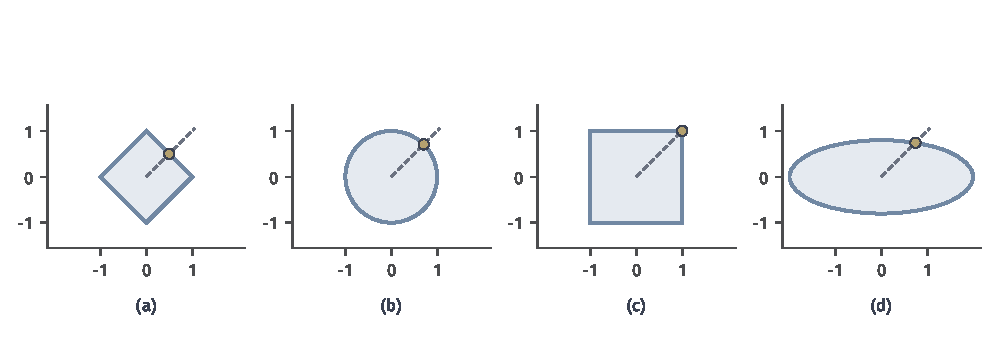
\includegraphics[width=169mm]{figures/00-shared/mathematical-preliminaries-upper/02-linear-spaces/matplotlib/ls-norm-unit-balls/ls-norm-unit-balls.pdf}
  \caption{三种范数的单位球。左：$\ell_1$单位球为菱形（累加绝对偏差）；中：$\ell_2$单位球为圆（欧氏长度）；右：$\ell_\infty$单位球为正方形（最大坐标偏差）。同一个点$(1,1)$的三种范数依次为$2$、$\sqrt2$、$1$。三者之间的倍数关系见第~\ref{sec:ls-error-scale-comparison}节。三图坐标尺度相同，为解析教学例。}
  \label{fig:ls-norm-unit-balls}
\end{figure*}

\subsubsection{范数的性质}
\label{sec:ls-p-norm-properties}

$1$、$2$、$\infty$范数的算法不同，却有几条共同的性质：大小非负，只有零向量的大小为零；向量放大$c$倍，大小变为$|c|$倍；两个向量之和的大小不超过各自大小之和。本小节对全部$p$范数证明这些性质，再比较不同$p$范数给出的大小最多相差多少倍。

\paragraph{非负性、正定性与齐次性}
这三条可以从公式直接读出。$\lVert\bm x\rVert_p$由绝对值汇总而成，总是非负；它为零当且仅当每个$|x_j|=0$，即$\bm x=\bm0$。

把$\bm x$换成$c\bm x$，每个$|x_j|$都乘以$|c|$。在$1\leq p<\infty$时，公式中的$p$次方与$1/p$次方相互抵消；在$p=\infty$时，最大值也乘以$|c|$。所以
\[
 \lVert c\bm x\rVert_p=|c|\,\lVert\bm x\rVert_p.
\]

\paragraph{三角不等式}
需要证明的只有三角不等式$\lVert\bm x+\bm y\rVert_p\leq\lVert\bm x\rVert_p+\lVert\bm y\rVert_p$。$p=1$和$p=\infty$时，它由实数的三角不等式逐坐标得到，见下面Minkowski不等式的证明。

$1<p<\infty$时，三角不等式要借助Hölder不等式。它用一对$p$范数与$q$范数控制两个向量逐坐标乘积之和，两个指数须满足共轭条件$1/p+1/q=1$。
\begin{theorem}[有限维Hölder不等式]
\label{thm:linear-algebra-holder}
设$\bm x,\bm y\in\mathbb R^d$，$1\leq p,q\leq\infty$且$1/p+1/q=1$（约定$1/\infty=0$），则
\begin{equation}
 |\bm x^\top\bm y|\leq\lVert\bm x\rVert_p\lVert\bm y\rVert_q.
 \label{eq:linear-algebra-holder}
\end{equation}
\end{theorem}
\begin{proof}
先设$1<p,q<\infty$，分三步证明。

第一步，证明Young不等式：对$u,v\geq0$，
\[
 uv\leq\frac{u^p}{p}+\frac{v^q}{q}.
\]
$u=0$时左侧为零，不等式成立。$u>0$时令$t=v/u^{p-1}\geq0$。由$1/p+1/q=1$得$(p-1)q=p$，于是
\[
 v^q=t^qu^{(p-1)q}=t^qu^p,\qquad uv=tu^p.
\]
代入后，不等式化为
\[
 u^p\Bigl(\frac1p+\frac{t^q}{q}-t\Bigr)\geq0.
\]
只需证明括号内的函数$f(t)=1/p+t^q/q-t$在$t\geq0$上非负。它的导数
\[
 f'(t)=t^{q-1}-1
\]
在$0<t<1$时为负、在$t>1$时为正，所以$f$在$t\geq0$上的最小值是
\[
 f(1)=\frac1p+\frac1q-1=0,
\]
不等式成立。

第二步，在单位尺度下求和。若$\bm x$或$\bm y$为零向量，结论两侧都为零。否则令$u_j=|x_j|/\lVert\bm x\rVert_p$、$v_j=|y_j|/\lVert\bm y\rVert_q$，则
\[
 \sum_ju_j^p=\sum_jv_j^q=1.
\]
对每个$j$用Young不等式再求和，得
\[
 \sum_ju_jv_j\leq\frac1p\sum_ju_j^p+\frac1q\sum_jv_j^q=\frac1p+\frac1q=1.
\]

第三步，恢复尺度。上式两边乘以$\lVert\bm x\rVert_p\lVert\bm y\rVert_q$，再用$|\bm x^\top\bm y|\leq\sum_j|x_j||y_j|$，即得
\[
 |\bm x^\top\bm y|\leq\sum_j|x_j||y_j|\leq\lVert\bm x\rVert_p\lVert\bm y\rVert_q.
\]

端点情形直接估计。$p=1$、$q=\infty$时，
\[
 \sum_j|x_j||y_j|\leq\Bigl(\max_j|y_j|\Bigr)\sum_j|x_j|=\lVert\bm x\rVert_1\lVert\bm y\rVert_\infty;
\]
$p=\infty$、$q=1$时交换两个向量的角色。
\end{proof}
$p=q=2$时，它给出$|\bm x^\top\bm y|\leq\lVert\bm x\rVert_2\lVert\bm y\rVert_2$。第~\ref{sec:ls-inner-product-definition}节将只用内积公理，对任一内积证明同样形式的不等式，即Cauchy--Schwarz不等式。

有了Hölder不等式，就可以对一般的$p$证明三角不等式。做法是把$|x_j+y_j|^p$拆成两个乘积之和，再对每一部分使用Hölder不等式。
\begin{theorem}[有限维Minkowski不等式]
\label{thm:linear-algebra-minkowski}
设$\bm x,\bm y\in\mathbb R^d$，$1\leq p\leq\infty$，则
\begin{equation}
 \lVert\bm x+\bm y\rVert_p\leq\lVert\bm x\rVert_p+\lVert\bm y\rVert_p.
 \label{eq:linear-algebra-minkowski}
\end{equation}
\end{theorem}
\begin{proof}
先处理两个端点。$p=1$时，对每个坐标使用实数的三角不等式，再求和，得到
\[
 \sum_j|x_j+y_j|\leq\sum_j|x_j|+\sum_j|y_j|.
\]
$p=\infty$时，对每个$j$都有
\[
 |x_j+y_j|\leq\lVert\bm x\rVert_\infty+\lVert\bm y\rVert_\infty.
\]
左侧对$j$取最大值，就得到所需结论。

下面设$1<p<\infty$。若$\bm x+\bm y=\bm0$，左侧为零，结论成立；以下设和向量非零。

取$q=p/(p-1)$，则$1/p+1/q=1$。先把每个坐标的$p$次方拆开，再用实数的三角不等式：
\[
 \begin{aligned}
 |x_j+y_j|^p
 &=|x_j+y_j|^{p-1}|x_j+y_j|\\
 &\leq |x_j+y_j|^{p-1}(|x_j|+|y_j|).
 \end{aligned}
\]
令$s_j=|x_j+y_j|^{p-1}$，把这些数排成向量$\bm s$。由于$(p-1)q=p$，它的$q$范数为
\[
 \begin{aligned}
 \lVert\bm s\rVert_q
 &=\Bigl(\sum_j|x_j+y_j|^p\Bigr)^{1/q}\\
 &=\lVert\bm x+\bm y\rVert_p^{p-1}.
 \end{aligned}
\]
把逐坐标的不等式求和，并对含$|x_j|$和含$|y_j|$的两部分分别使用Hölder不等式，得到
\[
 \begin{aligned}
 \lVert\bm x+\bm y\rVert_p^p
 &\leq\sum_js_j|x_j|+\sum_js_j|y_j|\\
 &\leq\lVert\bm s\rVert_q
       \bigl(\lVert\bm x\rVert_p+\lVert\bm y\rVert_p\bigr)\\
 &=\lVert\bm x+\bm y\rVert_p^{p-1}
       \bigl(\lVert\bm x\rVert_p+\lVert\bm y\rVert_p\bigr).
 \end{aligned}
\]
两边除以正数$\lVert\bm x+\bm y\rVert_p^{p-1}$，即得结论。
\end{proof}
所以每个$p$范数都满足三角不等式，特别是欧氏长度：两边之和不小于第三边。


\paragraph{范数的比较}
\phantomsection
\label{sec:ls-error-scale-comparison}

不同的$p$范数给同一个向量的大小不同。误差估计常常要在两种范数之间换算，因此需要知道它们最多相差多少倍。对$\mathbb R^d$中的坐标范数，这个倍数可以由有限求和直接算出。
\begin{theorem}[坐标范数的比较]
\label{thm:ls-coordinate-norm-comparison}
设$1\leq p\leq q\leq\infty$，约定$1/\infty=0$。对$\bm x\in\mathbb R^d$，
\begin{equation}
 \lVert\bm x\rVert_q\leq\lVert\bm x\rVert_p\leq d^{1/p-1/q}\lVert\bm x\rVert_q.
 \label{eq:ls-coordinate-norm-comparison}
\end{equation}
\end{theorem}
\begin{proof}
$\bm x=\bm0$时三项都为零，下设$\bm x\neq\bm0$。

左侧。令$\bm u=\bm x/\lVert\bm x\rVert_p$，则$\lVert\bm u\rVert_p=1$，所以每个$|u_j|\leq1$。$q=\infty$时这就是$\lVert\bm u\rVert_\infty\leq1$。

$q<\infty$时，由$|u_j|\leq1$与$q\geq p$得$|u_j|^q\leq|u_j|^p$。对$j$求和，得
\[
 \lVert\bm u\rVert_q^q\leq\lVert\bm u\rVert_p^p=1.
\]
两种情形都有$\lVert\bm u\rVert_q\leq1$，两边乘以$\lVert\bm x\rVert_p$即得。

右侧。$p=q$时两侧相同。$q=\infty$时，每一项$|x_j|^p$都不超过$\lVert\bm x\rVert_\infty^p$，于是
\[
 \sum_j|x_j|^p\leq d\,\lVert\bm x\rVert_\infty^p,
\]
开$p$次方即得。

设$p<q<\infty$，取$r=q/p>1$，其共轭指数满足$1/r'=1-p/q$。对向量$(|x_1|^p,\ldots,|x_d|^p)^\top$与全$1$向量使用Hölder不等式（定理~\ref{thm:linear-algebra-holder}），得
\[
 \begin{aligned}
 \sum_j|x_j|^p\cdot1
 &\leq\Bigl(\sum_j|x_j|^{q}\Bigr)^{p/q}d^{\,1-p/q}\\
 &=\lVert\bm x\rVert_q^p\,d^{\,1-p/q}.
 \end{aligned}
\]
两边开$p$次方，得
\[
 \lVert\bm x\rVert_p\leq d^{1/p-1/q}\lVert\bm x\rVert_q.
\]
\end{proof}
最常用的是$p,q\in\{1,2,\infty\}$的情形：
\[
 \begin{gathered}
 \lVert\bm x\rVert_\infty\leq\lVert\bm x\rVert_2\leq\sqrt d\,\lVert\bm x\rVert_\infty,\\
 \lVert\bm x\rVert_2\leq\lVert\bm x\rVert_1\leq\sqrt d\,\lVert\bm x\rVert_2,\\
 \lVert\bm x\rVert_\infty\leq\lVert\bm x\rVert_1\leq d\,\lVert\bm x\rVert_\infty.
 \end{gathered}
\]
下面在示例~\ref{ex:ls-p-norms}的向量上核对前两行。
\begin{example}[范数比较的数值核对]
\label{ex:ls-norm-comparison-check}
取$d=2$与$\bm x=(3,-4)^\top$。示例~\ref{ex:ls-p-norms}已经算出$\lVert\bm x\rVert_1=7$，$\lVert\bm x\rVert_2=5$，$\lVert\bm x\rVert_\infty=4$。代入前两行，比较常数分别为$\sqrt2$：
\[
 \begin{gathered}
 4\leq5\leq4\sqrt2\approx5.66,\\
 5\leq7\leq5\sqrt2\approx7.07.
 \end{gathered}
\]
四个不等式都成立，而且右侧的界离实际值不远。同一个误差$\bm x$在三种范数下读出$4$、$5$、$7$三个不同的数，比较定理保证的是这些读数之间的倍数不超过与维数有关的常数。
\end{example}
两侧的常数一般都不能改进，取等号的向量很简单。
\begin{example}[比较常数的取等]
\label{ex:ls-l1-linf-constants}
两个极端的向量分别使两侧取等号：只有一个非零坐标的$\bm e_1$，和各坐标一样大的全$1$向量$\bm 1$。

对每个$p$都有$\lVert\bm e_1\rVert_p=1$，所以$\bm e_1$使左侧取等号。

另一方面，全$1$向量的各范数为
\[
 \lVert\bm 1\rVert_p=d^{1/p}\quad(p<\infty),\qquad
 \lVert\bm 1\rVert_\infty=1.
\]
因此在约定$1/\infty=0$下总有
\[
 \lVert\bm 1\rVert_p=d^{1/p-1/q}\lVert\bm 1\rVert_q,
\]
右侧取等号。

大小全部集中在一个坐标上时，各范数读数相同；各坐标绝对值相等时，读数相差最大。例如$\ell_1$与$\ell_\infty$之间的常数$1$与$d$分别由$\bm e_1$和$\bm 1$达到，都不能改进。
\end{example}
右侧的常数随维数增长。维数较大时，换用范数带来的倍数差别不能在误差估计中忽略；固定维数下的比较式也不能当作对所有维数一致成立的界。

这里只比较了有明确公式的坐标范数。有限维空间上任意两个范数都只相差常数倍（定理~\ref{thm:ls-norm-equivalence}），这一结论的证明要用到闭有界集上连续函数的最值，在第~\ref{sec:multivariable-norm-equivalence}节给出。

本节建立了坐标向量的基本计算：加法、数乘与线性组合产生新的向量，欧氏内积把两个向量配成一个数，范数衡量向量的大小，满足非负性、正定性、齐次性与三角不等式，不同$p$范数之间只差与维数有关的常数倍。把若干向量并排放在一起，就得到下一节的矩阵。

% 矩阵一节：矩阵的表示与常见矩阵；加法与数乘、转置、矩阵与向量的乘积、矩阵乘法、逐项乘积（各自先定义、再整理性质）；初等行变换；逆矩阵；矩阵的幂。行列式、迹与Frobenius内积见下一节。

\section{矩阵}
\label{sec:ls-matrices}

一批样本的特征排成一张数表以后，常要对每个样本用同一组权重求加权和。矩阵就是这样的数表，矩阵乘法则一次写出这些加权和。

本节先规定矩阵的写法，再逐个讨论矩阵的运算，每种运算都先给定义、再整理性质。重点是矩阵乘法：它保留了实数乘法的结合律与分配律，却失去了交换律与消去律。最后三小节用乘法回答三个具体问题：怎样用可撤销的步骤化简矩阵，怎样撤销一次乘法，怎样记录同一矩阵的反复作用。

\subsection{矩阵的表示与常见矩阵}
\label{sec:ls-matrix-representation}

向量中的一个数用一个索引定位。数表中的一个数要由所在的行与列共同确定，需要两个索引。

\paragraph{矩阵、元素与形状}
$m$行$d$列的实数表称为矩阵（matrix），记为$\bm A\in\mathbb R^{m\times d}$。第$i$行、第$j$列的元素记为$\bm A_{i,j}$，不致混淆时也写作$a_{i,j}$。$m\times d$称为矩阵的形状，行数写在前，列数写在后。$\bm A_{i,:}$表示第$i$行，$\bm A_{:,j}$表示第$j$列，冒号表示取该方向上的全部位置；第$j$列是$m$维列向量，第$i$行是$d$维行向量。例如在
\[
 \bm A=\begin{bmatrix}1&2&3\\4&5&6\end{bmatrix}\in\mathbb R^{2\times3}
\]
中，$\bm A_{2,1}=4$，第一行$\bm A_{1,:}=\left[\begin{smallmatrix}1&2&3\end{smallmatrix}\right]$，第三列$\bm A_{:,3}=(3,6)^\top$。

两个矩阵相等，是指形状相同且每个对应元素相等。

只有一行的矩阵就是行向量，只有一列的矩阵就是列向量，所以向量可以看作矩阵的特例。

\paragraph{设计矩阵}
用矩阵记录数据时，通常让每行对应一个样本，每列对应一个特征，这样的矩阵称为设计矩阵。把示例~\ref{ex:ls-nearly-collinear-features}中的$\bm c_1,\bm c_2$并排作为两列，得到三个样本、两个特征的设计矩阵
\begin{equation}
\bm X_{\varepsilon}
 =\begin{bmatrix}\bm c_1&\bm c_2\end{bmatrix}
 =\begin{bmatrix}1&1\\1&1+\varepsilon\\1&1-\varepsilon\end{bmatrix},\qquad
 \bm c_2=\bm c_1+\varepsilon\bm q.
\label{eq:linear-algebra-nearly-collinear-design}
\end{equation}
后面各章反复用这个矩阵考察两列几乎相同时会出现什么问题。

\subsubsection{常见矩阵}
\label{sec:prelim-common-matrices}

有些矩阵的元素有固定的分布模式：大部分位置为零，或者关于主对角线对称。这些模式会让后面的运算大为简化。下面按元素的位置与取值逐类给出定义和例子；它们在矩阵乘法下呈现的固定模式，在第~\ref{sec:ls-common-matrix-products}节随乘法讨论。依赖内积的正交矩阵与正定矩阵在第~\ref{chap:normed-inner-product-spaces}章建立。

\paragraph{方阵}
行数等于列数的矩阵称为方阵（square matrix），$n\times n$方阵也称$n$阶方阵。位置$(i,i)$上的元素组成主对角线。例如
\[
 \begin{bmatrix}1&2\\3&4\end{bmatrix}
\]
是二阶方阵，主对角元素为$1$和$4$；$2\times3$矩阵不是方阵。下面的对角矩阵和三角矩阵都限定为方阵。

\paragraph{零矩阵}
全部元素都为$0$的矩阵称为零矩阵（zero matrix），记作$\bm0$。它不要求是方阵，需要时写明形状，例如
\[
 \bm0_{2\times3}=\begin{bmatrix}0&0&0\\0&0&0\end{bmatrix}.
\]

\paragraph{对角矩阵}
主对角线以外的元素都为$0$的方阵称为对角矩阵（diagonal matrix），记为$\operatorname{diag}(d_1,\ldots,d_n)$。主对角元素本身可以为$0$。例如
\[
\begin{gathered}
\operatorname{diag}(2,0)=\begin{bmatrix}2&0\\0&0\end{bmatrix},\\
\operatorname{diag}(1,-1,3)=\begin{bmatrix}1&0&0\\0&-1&0\\0&0&3\end{bmatrix}.
\end{gathered}
\]

\paragraph{单位矩阵}
主对角元素全为$1$的对角矩阵称为单位矩阵（identity matrix），记为$\bm I_n$；不必强调阶数时写作$\bm I$。它的第$j$列就是标准坐标向量$\bm e_j$。例如
\[
 \bm I_3=\begin{bmatrix}1&0&0\\0&1&0\\0&0&1\end{bmatrix}=\begin{bmatrix}\bm e_1&\bm e_2&\bm e_3\end{bmatrix}.
\]

\paragraph{上三角矩阵}
$i>j$时$\bm A_{i,j}=0$的方阵称为上三角矩阵（upper triangular matrix）。它的主对角线以下全为零，非零元素只可能出现在主对角线及其上方。例如
\[
 \begin{bmatrix}1&2&3\\0&4&5\\0&0&6\end{bmatrix}.
\]

\paragraph{下三角矩阵}
$i<j$时$\bm A_{i,j}=0$的方阵称为下三角矩阵（lower triangular matrix），它的主对角线以上全为零。例如
\[
 \begin{bmatrix}1&0&0\\2&3&0\\4&5&6\end{bmatrix}.
\]
对角矩阵既是上三角矩阵，也是下三角矩阵。

\paragraph{对称矩阵}
若方阵满足$\bm A_{i,j}=\bm A_{j,i}$对全部$i,j$成立，就称为对称矩阵（symmetric matrix）。它的元素关于主对角线镜像对称。定义转置以后，这个条件可以写作$\bm A^\top=\bm A$。例如
\[
\begin{bmatrix}1&2\\2&3\end{bmatrix},\qquad
\begin{bmatrix}4&-1&0\\-1&2&5\\0&5&1\end{bmatrix}.
\]
对角矩阵都是对称矩阵。

\paragraph{置换矩阵}
把单位矩阵的各列重新排列，得到的方阵称为置换矩阵（permutation matrix）。它的每行、每列恰有一个$1$，其余元素为$0$。例如
\[
\begin{bmatrix}0&1\\1&0\end{bmatrix}=\begin{bmatrix}\bm e_2&\bm e_1\end{bmatrix},\qquad
\begin{bmatrix}0&0&1\\1&0&0\\0&1&0\end{bmatrix}=\begin{bmatrix}\bm e_2&\bm e_3&\bm e_1\end{bmatrix}.
\]
定义矩阵乘法以后会看到，第一个矩阵乘在平面向量上，交换它的两个坐标。

\subsection{加法与数乘}
\label{sec:ls-matrix-addition-scaling}

矩阵的加法与数乘沿用向量的逐项规则。同形矩阵$\bm A,\bm B\in\mathbb R^{m\times n}$逐项相加减，数乘把每个元素乘以同一个实数$c$：
\[
 \begin{gathered}
(\bm A\pm\bm B)_{i,j}=a_{i,j}\pm b_{i,j},\\
(c\bm A)_{i,j}=ca_{i,j}.
 \end{gathered}
\]
结果的形状不变。下面是一组二阶矩阵的算例。
\begin{example}[矩阵的加法、减法与数乘]
\label{ex:ls-matrix-addition-scaling}
取
\[
\bm A=\begin{pmatrix}1&2\\3&4\end{pmatrix},\qquad
\bm B=\begin{pmatrix}0&1\\-1&2\end{pmatrix},\qquad
c=3.
\]
每个位置上的元素单独运算：
\[
\begin{gathered}
\bm A+\bm B=\begin{pmatrix}1&3\\2&6\end{pmatrix},\\
\bm A-\bm B=\begin{pmatrix}1&1\\4&2\end{pmatrix},\\
3\bm A=\begin{pmatrix}3&6\\9&12\end{pmatrix}.
\end{gathered}
\]
以$(2,1)$位置为例，$\bm A+\bm B$在这里是$3+(-1)=2$，$\bm A-\bm B$在这里是$3-(-1)=4$，都只用到$\bm A$与$\bm B$的$(2,1)$元。三个结果仍是$2\times2$矩阵，这和向量的逐坐标运算完全一样。
\end{example}
与向量一样，两个矩阵相加，要求形状相同、对应位置含义相同。$2\times3$矩阵与$3\times2$矩阵的元素个数相同，却不能相加。同形矩阵的线性组合按同样方式定义。

\subsubsection{加法与数乘的性质}
同形矩阵逐项相加与数乘，所以向量的八条规则在每个位置上照样成立。对同形矩阵$\bm A,\bm B,\bm C$和实数$a,b$，
\[
\begin{aligned}
 &\bm A+\bm B=\bm B+\bm A, && (\bm A+\bm B)+\bm C=\bm A+(\bm B+\bm C),\\
 &\bm A+\bm0=\bm A, && \bm A+(-\bm A)=\bm0,\\
 &a(b\bm A)=(ab)\bm A, && 1\bm A=\bm A,\\
 &(a+b)\bm A=a\bm A+b\bm A, && a(\bm A+\bm B)=a\bm A+a\bm B.
\end{aligned}
\]
每一条都可以在任一位置$(i,j)$上用实数运算直接验证。

\subsection{转置}
\label{sec:ls-matrix-transpose}

转置交换行与列：$\bm A\in\mathbb R^{m\times n}$的元素$a_{i,j}$原样搬到$\bm A^\top\in\mathbb R^{n\times m}$的位置$(j,i)$，
\[
 (\bm A^\top)_{j,i}=\bm A_{i,j}.
\]
形状随之交换，数值不变，原来的第$i$行成为第$i$列。把列向量看作$d\times1$矩阵，这一定义与上一节向量的转置一致。下面的例子显示行怎样变成列。
\begin{example}[转置一个$2\times3$矩阵]
\label{ex:ls-transpose-two-by-three}
把
\[
 \bm A=\begin{bmatrix}1&2&3\\4&5&6\end{bmatrix}\in\mathbb R^{2\times3}
\]
的每个$(i,j)$元搬到$(j,i)$位置，得到
\[
 \bm A^\top=\begin{bmatrix}1&4\\2&5\\3&6\end{bmatrix}\in\mathbb R^{3\times2}.
\]
$\bm A$的第一行$(1,2,3)$竖了起来，成为$\bm A^\top$的第一列；第二行$(4,5,6)$成为第二列。形状也随之由$2\times3$变为$3\times2$。
\end{example}

\subsubsection{转置的性质}

转置只改变元素的位置。下面两条说明它与加法、数乘的关系，以及转置两次的结果；它与矩阵乘积的关系要等定义了矩阵乘法以后，在第~\ref{sec:ls-reshaping}节讨论。

\paragraph{与加法、数乘交换}
\[
 \begin{gathered}
(\bm A+\bm B)^\top=\bm A^\top+\bm B^\top,\\
(c\bm A)^\top=c\bm A^\top.
 \end{gathered}
\]
转置只搬动元素，逐项运算的结果搬到新位置后不变。

\paragraph{转置的转置}
\[
 (\bm A^\top)^\top=\bm A.
\]
转置两次，$(i,j)$元先搬到$(j,i)$，再搬回$(i,j)$，每个元素回到原位。

\subsection{矩阵与向量的乘积}
\label{sec:prelim-matrix-records-prediction}

设$n$次观测的输入排成设计矩阵$\bm X\in\mathbb R^{n\times d}$，权重排成$\bm w\in\mathbb R^d$。线性预测对第$i$次观测计算加权和$\sum_j x_{i,j}w_j$，也就是$\bm X$的第$i$行与$\bm w$的内积。矩阵与向量的乘积把这$n$个加权和一次写出。对$\bm A\in\mathbb R^{m\times d}$与$\bm u\in\mathbb R^d$，$\bm A\bm u$是$m$维列向量，
\begin{equation}
(\bm A\bm u)_i=\sum_{j=1}^d\bm A_{i,j}u_j,\qquad i=1,\ldots,m.
\label{eq:prelim-matrix-prediction}
\end{equation}
这里矩阵的列数必须等于向量的维数。

同一个乘积可以按行算，也可以按列算，两者结果相同：
\begin{itemize}
 \item 按行算：输出的第$i$个坐标是第$i$行与$\bm u$的内积。
 \item 按列算：式~\eqref{eq:prelim-matrix-prediction}中，$u_j$乘的恰好是第$j$列的各个元素，所以
 \[
  \bm A\bm u=u_1\bm A_{:,1}+u_2\bm A_{:,2}+\cdots+u_d\bm A_{:,d},
 \]
 即乘积是矩阵各列以$u_j$为系数的线性组合。
\end{itemize}
按列算还说明，$\bm e_j$只有第$j$个系数为$1$，所以$\bm A\bm e_j=\bm A_{:,j}$：乘第$j$个标准坐标向量，就取出第$j$列。对贯穿例，按列算得$\bm X_\varepsilon\bm w=w_1\bm c_1+w_2\bm c_2$，预测是两个特征取值向量的线性组合。

下面用一个二阶例子核对两种算法给出同一结果。
\begin{example}[按行与按列计算矩阵与向量的乘积]
\label{ex:ls-matrix-vector-rows-columns}
取
\[
\bm A=\begin{bmatrix}2&1\\0&3\end{bmatrix},\qquad
\bm u=\begin{bmatrix}1\\1\end{bmatrix}.
\]
下面第一行算式按行算，每个坐标是$\bm A$的一行与$\bm u$的内积；第二行算式按列算，把$\bm A$的两列以$u_1=u_2=1$为系数组合起来：
\[
\begin{gathered}
\bm A\bm u
 =\begin{bmatrix}2\cdot1+1\cdot1\\0\cdot1+3\cdot1\end{bmatrix}
 =\begin{bmatrix}3\\3\end{bmatrix},\\
\bm A\bm u=1\begin{bmatrix}2\\0\end{bmatrix}+1\begin{bmatrix}1\\3\end{bmatrix}
 =\begin{bmatrix}3\\3\end{bmatrix}.
\end{gathered}
\]
两种算法都得到$(3,3)^\top$。按行算的每一项乘积，在按列算中也恰好出现一次，只是加起来的顺序不同。
\end{example}

用于数据时，一次矩阵与向量的乘积给出全部样本的预测。下面以一次函数为例。
\begin{example}[用矩阵与向量的乘积计算一次函数的取值与残差]
\label{ex:ls-affine-predictions}
设要在$x=1,2,3$三处计算一次函数$ax+b$的值。把三处的$x$排成第一列、再补上一列$1$，系数排成向量，即
\[
\bm X=\begin{pmatrix}1&1\\2&1\\3&1\end{pmatrix},\qquad
\bm w=\begin{pmatrix}a\\b\end{pmatrix}.
\]
按行算，
\[
 \bm X\bm w=\begin{pmatrix}1\cdot a+1\cdot b\\2\cdot a+1\cdot b\\3\cdot a+1\cdot b\end{pmatrix}=\begin{pmatrix}a+b\\2a+b\\3a+b\end{pmatrix}.
\]
$\bm X\bm w$的三个坐标正是三处的函数值；第二列全为$1$，使每行都加上同一个截距$b$。再把三处的观测输出排成$\bm y=(y_1,y_2,y_3)^\top$，全部残差就是$\bm X\bm w-\bm y$，平方误差总和写成
\[
 \sum_{i=1}^3\bigl(a\,i+b-y_i\bigr)^2
 =\lVert\bm X\bm w-\bm y\rVert_2^2.
\]
左侧逐处求函数值、减去观测、平方后相加；右侧把同样的计算写成残差向量长度的平方。

这里只用到乘积按行展开和长度的定义，与样本数、特征数无关。$n$个样本、$d$个特征时同样有
\[
 \sum_{i=1}^n\Bigl(\sum_{j=1}^d x_{i,j}w_j-y_i\Bigr)^2=\lVert\bm X\bm w-\bm y\rVert_2^2.
\]
于是一次矩阵与向量的乘积给出全部预测，平方误差总和则是残差向量长度的平方。
\end{example}

\subsection{矩阵乘法}
\label{sec:ls-matrix-operations}
\label{sec:ls-multiplication}
\label{sec:prelim-linear-actions-composition}

两次加权求和可能接连进行。设$\bm B\in\mathbb R^{d\times k}$，$\bm A\in\mathbb R^{m\times d}$。对$\bm x\in\mathbb R^k$，先算$\bm y=\bm B\bm x$，再算$\bm z=\bm A\bm y$。这就是两个映射的复合：$\bm x\mapsto\bm B\bm x$的输出$\bm y$恰好落在$\bm y\mapsto\bm A\bm y$的定义域$\mathbb R^d$中，复合映射把$\bm x$直接送到$\bm A(\bm B\bm x)$；映射复合的一般定义可参考\BookChapterRef{chap:sets-relations-maps}{卷一“集合、关系与映射”一章}。

逐坐标代入，再交换有限求和的次序，得到
\begin{equation}
 z_i=\sum_{\ell=1}^d a_{i,\ell}\sum_{j=1}^k b_{\ell,j}x_j
 =\sum_{j=1}^k\left(\sum_{\ell=1}^d a_{i,\ell}b_{\ell,j}\right)x_j.
 \label{eq:linear-algebra-matrix-product}
\end{equation}
可见$\bm z$仍是$\bm x$各坐标的加权和。把括号中的系数排成一张表，就得到矩阵乘法的定义。

对$\bm A\in\mathbb R^{m\times d}$与$\bm B\in\mathbb R^{d\times k}$，乘积$\bm A\bm B\in\mathbb R^{m\times k}$定义为
\begin{equation}
 (\bm A\bm B)_{i,j}=\sum_{\ell=1}^d\bm A_{i,\ell}\bm B_{\ell,j}.
 \label{eq:prelim-matrix-composition}
\end{equation}
左矩阵的列数必须等于右矩阵的行数。第$(i,j)$项取左矩阵的第$i$行与右矩阵的第$j$列，逐项相乘后相加。被求和掉的公共维数$d$，就是中间结果$\bm y$的维数。
$\bm B$只有一列时，式~\eqref{eq:prelim-matrix-composition}就是式~\eqref{eq:prelim-matrix-prediction}。两个向量的内积$\bm x^\top\bm y$是$1\times d$矩阵与$d\times1$矩阵的乘积，结果是$1\times1$矩阵，我们把它与其唯一的元素等同看待。

非方阵相乘时，写出每个因子的形状尤其有用。以$2\times3$矩阵乘$3\times2$矩阵为例，
\[
 \begin{aligned}
 &\begin{pmatrix}1&2&0\\0&1&3\end{pmatrix}
 \begin{pmatrix}1&0\\2&1\\1&-1\end{pmatrix}\\
 &=\begin{pmatrix}1\cdot1+2\cdot2+0\cdot1&1\cdot0+2\cdot1+0\cdot(-1)\\
 0\cdot1+1\cdot2+3\cdot1&0\cdot0+1\cdot1+3\cdot(-1)\end{pmatrix}\\
 &=\begin{pmatrix}5&2\\5&-2\end{pmatrix}.
 \end{aligned}
\]
左矩阵的列数与右矩阵的行数都是$3$，乘法有定义；输出保留左矩阵的$2$行和右矩阵的$2$列。若这两个数不相等，行与列就无法逐项配对。

\subsubsection{矩阵乘法的性质}
\label{sec:ls-matrix-operation-properties}

矩阵乘法保留了实数乘法的结合律和分配律，但一般不满足交换律和消去律。下面逐条核对，并检查每条规则对形状的要求。

\paragraph{单位乘}
\[
\bm I_m\bm A=\bm A=\bm A\bm I_d,\qquad
\bm A\in\mathbb R^{m\times d}.
\]
$\bm I_m$的第$i$行是$\bm e_i^\top$，它乘$\bm A$的第$j$列，取出$a_{i,j}$；右乘同理。单位矩阵在矩阵乘法中的作用，相当于数$1$在实数乘法中的作用。

\paragraph{零乘}
\[
 \bm0\bm A=\bm0,\qquad\bm A\bm0=\bm0.
\]
乘积的每个元素都是若干乘积之和。一个因子全为零时，每一项都为零。各个零矩阵的形状由相乘的另一个因子决定。

反过来不成立：由$\bm A\bm B=\bm0$不能推出$\bm A=\bm0$或$\bm B=\bm0$。下面是一个反例。
\begin{example}[反例：两个非零矩阵的乘积为零]
\label{ex:ls-zero-product-nonzero-factors}
两个二阶矩阵
\[
\bm A=\begin{bmatrix}1&0\\0&0\end{bmatrix},\qquad
\bm B=\begin{bmatrix}0&0\\1&0\end{bmatrix}
\]
各有一个非零元，都不是零矩阵。按定义相乘，
\[
 \bm A\bm B=\begin{bmatrix}1\cdot0+0\cdot1&1\cdot0+0\cdot0\\0\cdot0+0\cdot1&0\cdot0+0\cdot0\end{bmatrix}=\begin{bmatrix}0&0\\0&0\end{bmatrix}.
\]
四个元素全为零。可见两个非零因子的乘积可以是零矩阵，实数中“乘积为零则必有一个因子为零”的推理不能搬到矩阵上。
\end{example}
按列看可以说明原因。由乘积的元素公式，$\bm A\bm B$的第$j$列就是$\bm A$乘$\bm B$的第$j$列。所以$\bm A\bm B=\bm0$恰好意味着$\bm B$的每一列$\bm b$都满足$\bm A\bm b=\bm0$。上例中$\bm A$只保留第一个坐标、把第二个坐标清零；$\bm B$的第一列$(0,1)^\top$只有第二个坐标非零，第二列为零，于是两列都被$\bm A$清零。

\paragraph{结合律}
\[
 (\bm A\bm B)\bm C=\bm A(\bm B\bm C).
\]
按式~\eqref{eq:prelim-matrix-composition}展开，两边的第$(i,j)$项都是$\sum_k\sum_l a_{i,k}b_{k,l}c_{l,j}$，只是两个有限求和的次序不同。从映射的角度看，这就是复合的结合律：先作用$\bm C$、再作用$\bm B$、最后作用$\bm A$，无论先把哪两步合并，得到的都是同一个映射。取$\bm C$为列向量$\bm x$，得$(\bm A\bm B)\bm x=\bm A(\bm B\bm x)$：用乘积作用一次，等于先用$\bm B$、再用$\bm A$作用。这正是式~\eqref{eq:linear-algebra-matrix-product}引出乘法定义时的计算。有了结合律，多个形状相容的矩阵连乘时不必加括号。

\paragraph{分配律与数乘相容}
\[
 \begin{gathered}
\bm A(\bm B+\bm C)=\bm A\bm B+\bm A\bm C,\\
(\bm A+\bm B)\bm C=\bm A\bm C+\bm B\bm C,\\
c(\bm A\bm B)=(c\bm A)\bm B=\bm A(c\bm B).
 \end{gathered}
\]
逐项展开有限和即得。把右因子取为列向量，就得到矩阵与向量的乘积保持线性组合：
\begin{equation}
\bm A(a\bm u+b\bm v)=a\bm A\bm u+b\bm A\bm v,\qquad
\bm u,\bm v\in\mathbb R^d,\quad a,b\in\mathbb R.
\label{eq:prelim-matrix-linearity}
\end{equation}

由这一性质，函数$\bm u\mapsto\bm A\bm u$由它在$\bm e_1,\ldots,\bm e_d$上的输出完全确定。因为$\bm u=\sum_ju_j\bm e_j$，所以$\bm A\bm u=\sum_ju_j\bm A\bm e_j$，而这些输出$\bm A\bm e_j$就是$\bm A$的各列。第~\ref{chap:linear-representation}章把保持线性组合的函数称为线性映射，并说明每个这样的映射都能由一张矩阵记录。

\paragraph{分块乘法}
把矩阵按行、列切成尺寸相容的块，乘法公式对块照样成立。以$2\times2$分块为例，
\[
 \begin{bmatrix}\bm A_{1,1}&\bm A_{1,2}\\\bm A_{2,1}&\bm A_{2,2}\end{bmatrix}
 \begin{bmatrix}\bm B_{1,1}&\bm B_{1,2}\\\bm B_{2,1}&\bm B_{2,2}\end{bmatrix}
 =\begin{bmatrix}
  \bm A_{1,1}\bm B_{1,1}+\bm A_{1,2}\bm B_{2,1}&\bm A_{1,1}\bm B_{1,2}+\bm A_{1,2}\bm B_{2,2}\\
  \bm A_{2,1}\bm B_{1,1}+\bm A_{2,2}\bm B_{2,1}&\bm A_{2,1}\bm B_{1,2}+\bm A_{2,2}\bm B_{2,2}
 \end{bmatrix}.
\]
条件是每对相乘的块中，左块的列数等于右块的行数。理由如下：结果的每一块只用到左因子的一个行块和右因子的一个列块；式~\eqref{eq:prelim-matrix-composition}中对中间索引$\ell$的求和可以按列块分段进行，各段之和就是整段的和。块可以像数一样参与运算，只是块的次序不能交换。

把块分到最细，得到三种常用的特例。右因子按列分块，得$(\bm A\bm B)_{:,j}=\bm A\bm B_{:,j}$；左因子按行分块，得$(\bm A\bm B)_{i,:}=\bm A_{i,:}\bm B$；把中间维数$d$切成长度为$1$的$d$段，得到
\begin{equation}
 \bm A\bm B=\sum_{\ell=1}^d\bm A_{:,\ell}\bm B_{\ell,:},
 \label{eq:ls-product-outer-sum}
\end{equation}
其中一列$\bm A_{:,\ell}\in\mathbb R^{m\times1}$乘一行$\bm B_{\ell,:}\in\mathbb R^{1\times k}$，得到$(i,j)$元素为$a_{i,\ell}b_{\ell,j}$的$m\times k$矩阵。第~\ref{chap:matrix-approximation}章讨论低秩近似时，就从式~\eqref{eq:ls-product-outer-sum}出发。下面用一个二阶乘积核对这个公式。
\begin{example}[把乘积写成列乘行之和]
\label{ex:ls-product-as-outer-sum}
取
\[
\bm A=\begin{pmatrix}1&1\\0&1\end{pmatrix},\qquad
\bm B=\begin{pmatrix}1&0\\0&2\end{pmatrix}.
\]
$\bm A$的两列为$(1,0)^\top$与$(1,1)^\top$，$\bm B$的两行为$(1,0)$与$(0,2)$。把第$\ell$列与第$\ell$行配成一对相乘，再把两个结果相加：
\[
 \bm A\bm B=\begin{pmatrix}1\\0\end{pmatrix}\begin{pmatrix}1&0\end{pmatrix}+\begin{pmatrix}1\\1\end{pmatrix}\begin{pmatrix}0&2\end{pmatrix}
 =\begin{pmatrix}1&0\\0&0\end{pmatrix}+\begin{pmatrix}0&2\\0&2\end{pmatrix}=\begin{pmatrix}1&2\\0&2\end{pmatrix}.
\]
按式~\eqref{eq:prelim-matrix-composition}逐项计算$\bm A\bm B$，也得到同一个矩阵。两种算法的区别只在于：逐项计算先固定位置$(i,j)$、再对$\ell$求和，列乘行之和先固定$\ell$、一次写出所有位置上的贡献。
\end{example}

\paragraph{交换律不成立}
一般$\bm A\bm B\neq\bm B\bm A$。形状不同时，两个乘积不一定都有定义；即使两个因子是同阶方阵，两种次序的乘积也可能不同。下面是一个反例。
\begin{example}[反例：先交换再保留与先保留再交换]
\label{ex:ls-noncommuting-pair}
考虑两个作用很简单的二阶矩阵：$\bm P$只保留第一个坐标，$\bm S$交换两个坐标，
\[
\bm P=\begin{bmatrix}1&0\\0&0\end{bmatrix},\qquad
\bm S=\begin{bmatrix}0&1\\1&0\end{bmatrix}.
\]
按两种次序相乘，得到
\[
\bm P\bm S=\begin{bmatrix}0&1\\0&0\end{bmatrix},\qquad
\bm S\bm P=\begin{bmatrix}0&0\\1&0\end{bmatrix},
\]
所以$\bm P\bm S\neq\bm S\bm P$。看它们对$\bm u\in\mathbb R^2$的作用，差别的来源就清楚了：$\bm P\bm S\bm u=(u_2,0)^\top$是先交换、再保留第一个坐标，留下的是$u_2$；$\bm S\bm P\bm u=(0,u_1)^\top$是先保留、再交换，留下的是$u_1$，并且被移到了第二个位置。
\end{example}
书写$\bm A\bm B\bm x$时，作用顺序从右向左：先作用$\bm B$，后作用$\bm A$。

\paragraph{消去律不成立}
由$\bm A\bm B=\bm A\bm C$且$\bm A\neq\bm0$，不能推出$\bm B=\bm C$。原因是$\bm A\bm B=\bm A\bm C$等价于$\bm A(\bm B-\bm C)=\bm0$，而乘积为零推不出$\bm B-\bm C=\bm0$。下面用示例~\ref{ex:ls-zero-product-nonzero-factors}构造反例。
\begin{example}[反例：非零的左因子不能消去]
\label{ex:ls-cancellation-fails}
沿用示例~\ref{ex:ls-zero-product-nonzero-factors}中的
\[
\bm A=\begin{bmatrix}1&0\\0&0\end{bmatrix},\qquad
\bm B=\begin{bmatrix}0&0\\1&0\end{bmatrix},
\]
再取$\bm C=\bm0$。那个例子已经算出$\bm A\bm B=\bm0$，而零乘给出$\bm A\bm C=\bm0$，所以$\bm A\bm B=\bm A\bm C$。但$\bm B\neq\bm C$：尽管$\bm A\neq\bm0$，等式两边的$\bm A$也不能消去。
\end{example}
如果$\bm A$是可逆方阵（第~\ref{sec:prelim-inverse-matrices}节），在$\bm A\bm B=\bm A\bm C$两边左乘$\bm A^{-1}$，就得到$\bm B=\bm C$。所以可逆的左因子可以消去，一般的非零因子则不能。

\subsubsection{转置与乘积}
\label{sec:ls-reshaping}

第~\ref{sec:ls-matrix-transpose}节整理的转置性质只涉及加法、数乘和转置本身。乘法把左因子的行与右因子的列配对求和，而转置交换行与列，因此要单独考察乘积转置以后两个因子怎样排列。下面先给出这条规则，再看它在内积和对称性上的两个推论。

\paragraph{乘积的转置}
\[
 (\bm A\bm B)^\top=\bm B^\top\bm A^\top.
\]
乘积转置以后，因子的次序反过来。按元素公式，
\[
 \begin{aligned}
 \bigl((\bm A\bm B)^\top\bigr)_{i,j}
 &=(\bm A\bm B)_{j,i}\\
 &=\sum_\ell a_{j,\ell}b_{\ell,i}\\
 &=\sum_\ell(\bm B^\top)_{i,\ell}(\bm A^\top)_{\ell,j}\\
 &=(\bm B^\top\bm A^\top)_{i,j}.
 \end{aligned}
\]
多个因子时依次使用这条规则，得$(\bm A\bm B\bm C)^\top=\bm C^\top\bm B^\top\bm A^\top$。

\paragraph{内积中的转置}
\[
\langle\bm A\bm x,\bm y\rangle=\langle\bm x,\bm A^\top\bm y\rangle,\qquad
\bm A\in\mathbb R^{m\times d},\ \bm x\in\mathbb R^d,\ \bm y\in\mathbb R^m.
\]
由上一条，$(\bm A\bm x)^\top\bm y=\bm x^\top\bm A^\top\bm y$。所以在欧氏内积中，作用在左侧向量上的$\bm A$，可以改写成作用在右侧向量上的$\bm A^\top$。

\paragraph{$\bm A^\top\bm A$对称}
对任意矩阵$\bm A$，$\bm A^\top\bm A$与$\bm A\bm A^\top$都是对称矩阵。由乘积的转置，$(\bm A^\top\bm A)^\top=\bm A^\top(\bm A^\top)^\top=\bm A^\top\bm A$；另一个同理。下面直接算出一个$\bm A\bm A^\top$。
\begin{example}[计算$\bm A\bm A^\top$]
\label{ex:ls-gram-product-symmetric}
取
\[
 \bm A=\begin{bmatrix}1&2&3\\4&5&6\end{bmatrix}.
\]
$\bm A^\top$的第$j$列就是$\bm A$的第$j$行，所以$\bm A\bm A^\top$的$(i,j)$元是$\bm A$的第$i$行与第$j$行的内积：
\[
 \bm A\bm A^\top=\begin{bmatrix}1+4+9&4+10+18\\4+10+18&16+25+36\end{bmatrix}=\begin{bmatrix}14&32\\32&77\end{bmatrix}.
\]
$(1,2)$元与$(2,1)$元都是第一、二两行的内积$32$；内积与两行的先后无关，所以结果必然对称。对角元$14$、$77$则是两行各自长度的平方。
\end{example}

\subsubsection{常见矩阵的乘法}
\label{sec:ls-common-matrix-products}

第~\ref{sec:prelim-common-matrices}节的几类常见矩阵参与乘法时，结果有固定的模式。下面逐类说明。

\paragraph{对角矩阵的乘法}
设$\bm D=\operatorname{diag}(d_1,\ldots,d_n)$。左乘和右乘对角矩阵分别给出
\[
 \begin{gathered}
(\bm D\bm A)_{i,j}=d_i\bm A_{i,j},\\
(\bm A\bm D)_{i,j}=\bm A_{i,j}d_j.
 \end{gathered}
\]
乘积公式中，左乘时只剩$\ell=i$一项，右乘时只剩$\ell=j$一项。所以左乘对角矩阵缩放各行，右乘缩放各列。作用在向量上，$\bm D\bm u=(d_1u_1,\ldots,d_nu_n)^\top$是逐坐标缩放。两个对角矩阵相乘时，对角元逐个相乘：
\[
 \operatorname{diag}(d_1,\ldots,d_n)\operatorname{diag}(e_1,\ldots,e_n)=\operatorname{diag}(d_1e_1,\ldots,d_ne_n).
\]
因此对角矩阵之间可以交换次序。下面的例子比较左乘与右乘。
\begin{example}[左乘与右乘对角矩阵]
\label{ex:ls-diagonal-scaling}
取
\[
\bm D=\operatorname{diag}(2,3),\qquad
\bm A=\begin{bmatrix}1&2\\3&4\end{bmatrix},
\]
把$\bm D$分别放在$\bm A$的左边和右边：
\[
 \begin{aligned}
 \bm D\bm A&=\begin{bmatrix}2\cdot1&2\cdot2\\3\cdot3&3\cdot4\end{bmatrix}=\begin{bmatrix}2&4\\9&12\end{bmatrix},\\
 \bm A\bm D&=\begin{bmatrix}1\cdot2&2\cdot3\\3\cdot2&4\cdot3\end{bmatrix}=\begin{bmatrix}2&6\\6&12\end{bmatrix}.
 \end{aligned}
\]
左乘把第一、二行分别乘以$2$、$3$，右乘则把第一、二列分别乘以$2$、$3$。两个结果不同：对角矩阵彼此可以交换，与一般矩阵相乘时仍要区分左右。
\end{example}

\paragraph{三角矩阵的乘法}
若$\bm A,\bm B$都是$n$阶上三角矩阵，则$\bm A\bm B$也是上三角矩阵，并且
\[
 (\bm A\bm B)_{i,i}=\bm A_{i,i}\bm B_{i,i}.
\]
理由如下。在$(\bm A\bm B)_{i,j}=\sum_\ell\bm A_{i,\ell}\bm B_{\ell,j}$中，$\bm A_{i,\ell}$只在$\ell\geq i$时可能非零，$\bm B_{\ell,j}$只在$\ell\leq j$时可能非零，所以只有$i\leq\ell\leq j$的项可能非零。$i>j$时没有这样的$\ell$，乘积元素为零；$i=j$时只剩$\ell=i$一项。下三角矩阵同理：两个下三角矩阵的乘积仍是下三角矩阵，对角元逐个相乘。下面是一个二阶算例。
\begin{example}[两个上三角矩阵的乘积]
\label{ex:ls-upper-triangular-product}
取两个上三角矩阵
\[
\bm A=\begin{bmatrix}1&2\\0&3\end{bmatrix},\qquad
\bm B=\begin{bmatrix}4&5\\0&6\end{bmatrix}.
\]
它们的乘积为
\[
 \bm A\bm B=\begin{bmatrix}1\cdot4+2\cdot0&1\cdot5+2\cdot6\\0\cdot4+3\cdot0&0\cdot5+3\cdot6\end{bmatrix}=\begin{bmatrix}4&17\\0&18\end{bmatrix}.
\]
左下角的$0\cdot4+3\cdot0$中，每一项都有一个因子取自主对角线以下的零，所以乘积仍是上三角矩阵。对角元$4=1\cdot4$、$18=3\cdot6$只是两个因子对角元的乘积；右上角的$17$则同时用到了两个因子的非对角元，没有这样简单的规律。
\end{example}

\paragraph{置换矩阵的乘法}
设$\bm P=\left[\begin{smallmatrix}\bm e_{\sigma(1)}&\cdots&\bm e_{\sigma(n)}\end{smallmatrix}\right]$，其中$\sigma$是$\{1,\ldots,n\}$上的排列，则
\[
 \begin{gathered}
(\bm P\bm A)_{\sigma(i),:}=\bm A_{i,:},\\
(\bm A\bm P)_{:,j}=\bm A_{:,\sigma(j)}.
 \end{gathered}
\]
也就是说，左乘$\bm P$把$\bm A$的第$i$行移到第$\sigma(i)$行；右乘$\bm P$后，第$j$列取自$\bm A$的第$\sigma(j)$列。例如二阶置换矩阵
\[
 \begin{bmatrix}0&1\\1&0\end{bmatrix}
\]
左乘交换两行，右乘交换两列。

两个置换矩阵的乘积仍是置换矩阵。设$\bm P'$是另一个置换矩阵，则$\bm P'\bm P$的第$j$列是$\bm P'\bm e_{\sigma(j)}$，即$\bm P'$的第$\sigma(j)$列。不同的$j$取到$\bm P'$的不同列，所以$\bm P'\bm P$的各列是互不相同的标准坐标向量，它是单位矩阵各列的一种重排。

\paragraph{对称矩阵的乘积}
若$\bm A,\bm B$是同阶对称矩阵，则
\[
 (\bm A\bm B)^\top=\bm B^\top\bm A^\top=\bm B\bm A,
\]
所以$\bm A\bm B$对称当且仅当$\bm A\bm B=\bm B\bm A$。两个对称矩阵一般不交换，它们的乘积一般也不对称。下面是一个反例。
\begin{example}[反例：两个对称矩阵的乘积不对称]
\label{ex:ls-symmetric-product-not-symmetric}
取两个对称矩阵
\[
\bm A=\begin{bmatrix}1&1\\1&0\end{bmatrix},\qquad
\bm B=\operatorname{diag}(1,2).
\]
右乘对角矩阵$\bm B$相当于把$\bm A$的第二列乘以$2$，
\[
 \bm A\bm B=\begin{bmatrix}1\cdot1&1\cdot2\\1\cdot1&0\cdot2\end{bmatrix}=\begin{bmatrix}1&2\\1&0\end{bmatrix}.
\]
原来关于主对角线对称的两个$1$，只有右上角的一个被放大，于是$(\bm A\bm B)_{1,2}=2\neq1=(\bm A\bm B)_{2,1}$，乘积不对称。这与上面的判据一致：换成左乘，$\bm B$放大的是第二行，
\[
 \bm B\bm A=\begin{bmatrix}1&1\\2&0\end{bmatrix}\neq\bm A\bm B,
\]
两个因子不交换。
\end{example}

\subsection{逐项乘积}
\label{sec:ls-hadamard-product}

矩阵乘法对公共索引求和。另一种常用的“乘积”不对任何索引求和，只把两个同形数组在同一位置上的元素相乘。

设$\bm A,\bm B\in\mathbb R^{m\times n}$，它们的\term{逐元素乘积}（Hadamard product）记作$\bm A\odot\bm B$，
\begin{equation}
 (\bm A\odot\bm B)_{i,j}=a_{i,j}b_{i,j}.
 \label{eq:ls-hadamard}
\end{equation}
输出仍是$m\times n$矩阵。同维向量和更高阶的同形数组也按同样的方式逐项相乘。

对同样两个矩阵，两种乘积的结果完全不同。
\begin{example}[逐项乘积与矩阵乘积的对比]
\label{ex:ls-hadamard-vs-matrix-product}
取
\[
\bm A=\begin{bmatrix}1&2\\3&4\end{bmatrix},\qquad
\bm B=\begin{bmatrix}0&1\\1&0\end{bmatrix},
\]
其中$\bm B$是交换两个坐标的置换矩阵。分别计算两种乘积：
\[
 \begin{aligned}
 \bm A\odot\bm B&=\begin{bmatrix}1\cdot0&2\cdot1\\3\cdot1&4\cdot0\end{bmatrix}=\begin{bmatrix}0&2\\3&0\end{bmatrix},\\
 \bm A\bm B&=\begin{bmatrix}1\cdot0+2\cdot1&1\cdot1+2\cdot0\\3\cdot0+4\cdot1&3\cdot1+4\cdot0\end{bmatrix}=\begin{bmatrix}2&1\\4&3\end{bmatrix}.
 \end{aligned}
\]
逐项乘积保留$\bm A$在$\bm B$取$1$处的元素，把$\bm B$为零的位置置零；矩阵乘积则是右乘置换矩阵，交换了$\bm A$的两列。两个结果在每个位置上都不同。
\end{example}
固定一个掩码矩阵$\bm M$，运算$\bm X\mapsto\bm M\odot\bm X$把$\bm M$为零的位置置零，把其余位置按$\bm M$的元素缩放。因此逐项乘积适合表达“挑选或调制另一个数组”。

\subsubsection{逐项乘积的性质}

逐项乘积在每个位置上只是实数乘法，所以它的规则都可以逐个位置从实数运算推出。以下矩阵的形状都相同。

\paragraph{交换律}
\[
 \bm A\odot\bm B=\bm B\odot\bm A.
\]
式~\eqref{eq:ls-hadamard}右端是实数乘法，逐个位置验证即得。逐项乘积可交换，矩阵乘积不可交换，这再次说明两者是不同的运算。

\paragraph{结合律}
\[
 (\bm A\odot\bm B)\odot\bm C=\bm A\odot(\bm B\odot\bm C),
\]
两边的$(i,j)$元素都是$a_{i,j}b_{i,j}c_{i,j}$。

\paragraph{分配律}
\[
 \bm A\odot(\bm B+\bm C)=\bm A\odot\bm B+\bm A\odot\bm C,
\]
两边的$(i,j)$元素都是$a_{i,j}(b_{i,j}+c_{i,j})$。

\paragraph{单位元是全$1$数组}
全部元素为$1$的同形数组$\bm J$满足$\bm J\odot\bm A=\bm A$。单位矩阵不是逐项乘积的单位元：$\bm I_2\odot\bm A$只保留$\bm A$的对角元，把非对角元都变为零。

\paragraph{对每个因子分别线性}
固定一个因子$\bm M$时，$\bm X\mapsto\bm M\odot\bm X$保持线性组合。两个因子都可变时，乘积只对每个因子分别线性，对两者整体不是线性的：同时把两个因子放大两倍，结果放大四倍。第~\ref{chap:linear-representation}章还会看到，换一组记录方向以后，矩阵乘积所表示的复合关系保持不变，逐项乘积的结果则随记录方式改变。

\subsection{初等行变换}
\label{sec:ls-elementary-row-operations}

解方程和求逆时，需要把一个矩阵逐步化成容易辨认的形式。每一步都应当可以撤销，这样才不会丢失原矩阵中的信息。为此，对矩阵的行只允许三种\term{初等行变换}（elementary row operation）。下面用$r_i$表示第$i$行，并用同一个矩阵
\[
 \bm A=\begin{bmatrix}1&2\\3&4\\5&6\end{bmatrix}
\]
分别演示。每种变换都可以写成左乘一个矩阵：对单位矩阵执行同一变换，所得矩阵称为\term{初等矩阵}（elementary matrix），记为$\bm E$，那么$\bm E\bm A$恰好是对$\bm A$执行这一变换的结果。

第一种是交换两行，记作$r_i\leftrightarrow r_k$。它只改变行的先后，不改变任何一行的内容。图~\ref{fig:ls-row-swap}交换$\bm A$的第$1$、$3$行，对应的初等矩阵是交换$\bm I_3$第$1$、$3$行所得的置换矩阵。再交换一次同样的两行，就回到原矩阵，所以这种变换的逆就是它自己。
\begin{figure}[!htb]
  \centering
  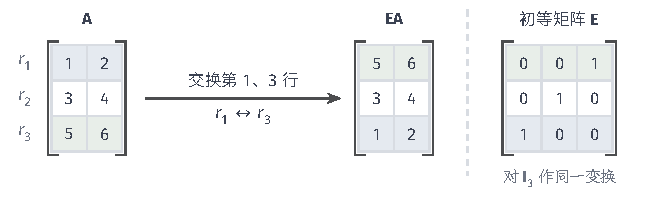
\includegraphics[width=109mm]{figures/02-vectors-matrices-and-multivariate-calculus/01-vectors-and-linear-spaces/tikz/ls-elementary-row-operations/row-swap.pdf}
  \caption{交换两行。左为$\bm A$，中间为交换第$1$、$3$行后的$\bm E\bm A$，右为对$\bm I_3$作同一交换得到的初等矩阵$\bm E$；同色表示同一行内容，换位后颜色随行移动。}
  \label{fig:ls-row-swap}
\end{figure}

第二种是将一行乘以非零数$c$，记作$r_i\leftarrow cr_i$。它把这一行的每个元素放大$c$倍，其余行不动。图~\ref{fig:ls-row-scale}把第$2$行乘以$2$，对应的初等矩阵是对角矩阵$\operatorname{diag}(1,2,1)$。要撤销它，只需把同一行乘以$1/c$。这里必须要求$c\neq0$：乘以$0$会把整行抹成零，原来的数据无法恢复。
\begin{figure}[!htb]
  \centering
  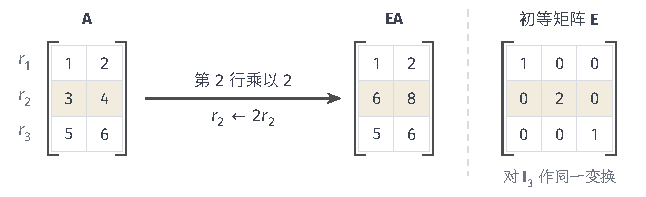
\includegraphics[width=109mm]{figures/02-vectors-matrices-and-multivariate-calculus/01-vectors-and-linear-spaces/tikz/ls-elementary-row-operations/row-scale.pdf}
  \caption{一行乘以非零数。第$2$行（黄色）乘以$2$，其余两行不变；初等矩阵$\bm E=\operatorname{diag}(1,2,1)$只在第$2$个对角元上与$\bm I_3$不同。}
  \label{fig:ls-row-scale}
\end{figure}

第三种是将一行加上另一行的倍数，记作$r_i\leftarrow r_i+cr_k$（$i\neq k$）。被加的一行改变，提供倍数的一行保持不动。图~\ref{fig:ls-row-replace}把第$3$行加上第$1$行的$-5$倍，第$3$行的首个元素$5$变成$0$；后面消元时正是用这种变换把指定位置化为零。对应的初等矩阵是在$\bm I_3$的$(3,1)$位置放上$-5$。撤销时，把第$3$行再加上第$1$行的$5$倍：第$1$行没有变，所以原来加上的量可以原样减回。
\begin{figure}[!htb]
  \centering
  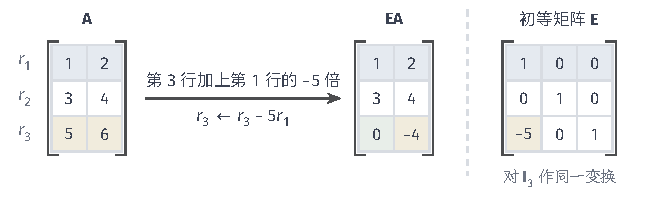
\includegraphics[width=109mm]{figures/02-vectors-matrices-and-multivariate-calculus/01-vectors-and-linear-spaces/tikz/ls-elementary-row-operations/row-replace.pdf}
  \caption{一行加上另一行的倍数。第$3$行（黄色）加上第$1$行（蓝色）的$-5$倍，第$1$行不变，第$3$行首个元素化为$0$（绿色）；初等矩阵$\bm E$只在$(3,1)$位置与$\bm I_3$不同。}
  \label{fig:ls-row-replace}
\end{figure}

三种变换的逆操作仍是同类的初等行变换，对应的初等矩阵就是$\bm E$的逆，所以每个初等矩阵都可逆。接连执行若干次行变换，相当于依次左乘这些初等矩阵，总的效果是左乘它们的乘积，它仍是可逆矩阵。

用初等行变换把矩阵化为阶梯形、求解线性方程组和求逆矩阵的具体做法，放在第~\ref{sec:ls-gaussian-elimination}节与求解方法一起讨论。

\subsection{逆矩阵}
\label{sec:prelim-inverse-matrices}

逆矩阵用来撤销一次矩阵乘法。对$n$阶方阵$\bm A$，若存在$n$阶方阵$\bm B$满足
\[
 \bm A\bm B=\bm B\bm A=\bm I_n,
\]
就称$\bm A$可逆，称$\bm B$为$\bm A$的\term{逆矩阵}（inverse matrix），记作$\bm A^{-1}$。

可逆矩阵给出的方程有唯一解。设$\bm A$可逆。若$\bm A\bm x=\bm y$，两边左乘$\bm A^{-1}$得$\bm x=\bm A^{-1}\bm y$，所以方程至多有一个解；反过来，$\bm x=\bm A^{-1}\bm y$满足$\bm A\bm x=\bm A\bm A^{-1}\bm y=\bm y$。所以方程$\bm A\bm x=\bm y$有唯一解$\bm x=\bm A^{-1}\bm y$。

逆矩阵若存在则唯一。若$\bm B,\bm C$都满足条件，由结合律，
\[
 \bm B=\bm B(\bm A\bm C)=(\bm B\bm A)\bm C=\bm C.
\]
因此记号$\bm A^{-1}$没有歧义。

怎样求逆取决于矩阵的结构。下面先给出对角矩阵和二阶方阵的逆，再说明一般方阵的求逆怎样归结为解方程。

\paragraph{对角矩阵的逆}
每个$d_i\neq0$时，逐个取倒数：
\[
 \operatorname{diag}(d_1,\ldots,d_n)^{-1}=\operatorname{diag}(1/d_1,\ldots,1/d_n).
\]
两个对角矩阵相乘时对角元逐个相乘，所以两侧乘积都是$\bm I_n$。例如$\operatorname{diag}(2,1)^{-1}=\operatorname{diag}(1/2,1)$。若某个$d_i=0$，则$\bm D=\operatorname{diag}(d_1,\ldots,d_n)$左乘任何$\bm B$，都把$\bm B$的第$i$行乘以$0$。于是$\bm D\bm B$的第$i$行是零，不可能等于$\bm I_n$的第$i$行，这时$\bm D$不可逆。

\paragraph{二阶方阵的逆}
$ad-bc\neq0$时，
\[
 \begin{pmatrix}a&b\\c&d\end{pmatrix}^{-1}=\frac1{ad-bc}\begin{pmatrix}d&-b\\-c&a\end{pmatrix}.
\]
直接相乘即可验证两侧乘积都是$\bm I_2$：例如左上元素为$(ad-bc)/(ad-bc)=1$，右上元素为$(-ab+ba)/(ad-bc)=0$。分母$ad-bc$就是下一节的二阶行列式。

\paragraph{一般方阵的逆}
一般方阵没有这样简短的公式。按列看等式$\bm A\bm A^{-1}=\bm I_n$，$\bm A^{-1}$的第$j$列$\bm A^{-1}\bm e_j$正是方程$\bm A\bm x=\bm e_j$的解，所以求逆就是解$n$个系数矩阵相同的线性方程组。怎样用初等行变换一并解这些方程，以及化简失败为什么说明矩阵不可逆，在第~\ref{sec:ls-gaussian-elimination}节讨论；方阵何时可逆，在第~\ref{chap:linear-solution-selection}章系统处理。只求一个方程的解时，通常直接消元或用分解求解，不必先求出整个逆矩阵。

\paragraph{单侧逆}
矩形矩阵没有双侧的逆，但可能从一侧抵消。对$\bm A\in\mathbb R^{m\times d}$，满足$\bm L\bm A=\bm I_d$的$\bm L\in\mathbb R^{d\times m}$称为左逆，满足$\bm A\bm R=\bm I_m$的$\bm R\in\mathbb R^{d\times m}$称为右逆。

两种单侧逆对方程$\bm A\bm x=\bm y$的作用不同。有左逆时，若方程有解，两边左乘$\bm L$得$\bm x=\bm L\bm y$，所以解只能是$\bm L\bm y$。有右逆时，$\bm A(\bm R\bm y)=\bm I_m\bm y=\bm y$，所以$\bm x=\bm R\bm y$总是一个解。

与方阵的逆不同，单侧逆一般不唯一。
\begin{example}[反例：左逆不唯一]
\label{ex:ls-left-inverse-not-unique}
取$\bm A=(1,0)^\top\in\mathbb R^{2\times1}$。对任意实数$c$，令$\bm L=(1,c)\in\mathbb R^{1\times2}$，则
\[
 \bm L\bm A=1\cdot1+c\cdot0=1=\bm I_1.
\]
$\bm A$的第二个坐标是零，$\bm L$的第二个元素无论取什么都不影响乘积。于是每个$c$都给出一个左逆，$\bm A$的左逆有无穷多个。
\end{example}

回到方阵。下面几条规则说明，可逆方阵经过乘积、求逆、数乘和转置以后仍然可逆，并给出逆矩阵的表达式。设$\bm A,\bm B$都是$n$阶可逆方阵。

\paragraph{乘积的逆}
两个可逆方阵的乘积仍然可逆，它的逆是两个因子的逆按相反次序相乘。
\begin{theorem}[乘积的逆]
\label{thm:ls-inverse-product}
设$\bm A,\bm B$都是$n$阶可逆方阵，则$\bm A\bm B$可逆，且
\begin{equation}
 (\bm A\bm B)^{-1}=\bm B^{-1}\bm A^{-1}.
 \label{eq:ls-inverse-product}
\end{equation}
\end{theorem}
\begin{proof}
由矩阵乘法的结合律，
\[
 \begin{gathered}
 (\bm A\bm B)(\bm B^{-1}\bm A^{-1})=\bm A(\bm B\bm B^{-1})\bm A^{-1}=\bm A\bm A^{-1}=\bm I_n,\\
 (\bm B^{-1}\bm A^{-1})(\bm A\bm B)=\bm B^{-1}(\bm A^{-1}\bm A)\bm B=\bm B^{-1}\bm B=\bm I_n.
 \end{gathered}
\]
按逆矩阵的定义，$\bm B^{-1}\bm A^{-1}$是$\bm A\bm B$的逆；由逆矩阵的唯一性，式~\eqref{eq:ls-inverse-product}成立。
\end{proof}
次序反转是因为$\bm A\bm B\bm x$先作用$\bm B$、再作用$\bm A$，撤销时要先撤销后作用的$\bm A$，再撤销$\bm B$。

\paragraph{逆的逆}
\[
 (\bm A^{-1})^{-1}=\bm A.
\]
在定义中，$\bm A$与$\bm A^{-1}$的地位对称：$\bm A^{-1}\bm A=\bm A\bm A^{-1}=\bm I_n$同样说明$\bm A$是$\bm A^{-1}$的逆。

\paragraph{数乘的逆}
\[
 (c\bm A)^{-1}=c^{-1}\bm A^{-1}\qquad(c\neq0).
\]
直接相乘：$(c\bm A)(c^{-1}\bm A^{-1})=(cc^{-1})\bm A\bm A^{-1}=\bm I_n$，反方向同理。

\paragraph{转置的逆}
\[
 (\bm A^\top)^{-1}=(\bm A^{-1})^\top.
\]
由乘积的转置，$\bm A^\top(\bm A^{-1})^\top=(\bm A^{-1}\bm A)^\top=\bm I^\top=\bm I$，反方向同理，所以$(\bm A^{-1})^\top$就是$\bm A^\top$的逆。

\subsection{矩阵的幂}
\label{sec:ls-matrix-power-rules}

同一个方阵反复作用，就得到矩阵的幂。对$d$阶方阵$\bm A$，$\bm A^k$定义为$k$个$\bm A$连乘（$k\geq1$），并规定$\bm A^0=\bm I_d$。$\bm A$可逆时，再定义负幂$\bm A^{-k}=(\bm A^{-1})^k$。非方阵不能与自身相乘，所以没有矩阵幂。

矩阵的幂是反复的矩阵乘法，不是逐元素乘方。下面的例子说明两者的差别。
\begin{example}[矩阵的平方不是逐元素平方]
\label{ex:ls-matrix-square-shear}
取
\[
 \bm A=\begin{pmatrix}1&1\\0&1\end{pmatrix},
\]
按矩阵乘法计算它的平方：
\[
 \bm A^2=\begin{pmatrix}1&1\\0&1\end{pmatrix}\begin{pmatrix}1&1\\0&1\end{pmatrix}
 =\begin{pmatrix}1\cdot1+1\cdot0&1\cdot1+1\cdot1\\0\cdot1+1\cdot0&0\cdot1+1\cdot1\end{pmatrix}
 =\begin{pmatrix}1&2\\0&1\end{pmatrix}.
\]
右上角的元素变为$2$，逐元素平方却只会得到$1^2=1$。差别在于$\bm A^2$的右上角是第一行与第二列的内积$1\cdot1+1\cdot1$，同时用到了两个元素。继续相乘，右上角每次增加$1$。
\end{example}

有两类矩阵由幂的关系刻画。满足$\bm A^2=\bm A$的方阵称为\term{幂等}（idempotent）矩阵，它作用一次与作用多次效果相同。存在正整数$s$使$\bm N^s=\bm0$的方阵称为\term{幂零}（nilpotent）矩阵。下面各举一例。
\begin{example}[幂等矩阵与幂零矩阵]
\label{ex:ls-idempotent-nilpotent}
看两个二阶矩阵
\[
\bm P=\operatorname{diag}(1,0),\qquad
\bm N=\begin{pmatrix}0&1\\0&0\end{pmatrix}
\]
对$\bm u\in\mathbb R^2$的作用。$\bm P\bm u=(u_1,0)^\top$只保留第一个坐标；$(u_1,0)^\top$再经过$\bm P$，第一个坐标照样保留，第二个坐标本来就是零，结果不变，所以$\bm P^2=\bm P$。$\bm N\bm u=(u_2,0)^\top$把第二个坐标移到第一个位置，并把第二个位置清零；再作用一次时，$\bm N$丢掉第一个坐标$u_2$，而第二个坐标已是零，得$\bm N(u_2,0)^\top=(0,0)^\top$。直接相乘也得到
\[
 \bm N^2=\begin{pmatrix}0&1\\0&0\end{pmatrix}\begin{pmatrix}0&1\\0&0\end{pmatrix}=\begin{pmatrix}0&0\\0&0\end{pmatrix}.
\]
所以$\bm P$是幂等矩阵；$\bm N$本身不是零矩阵，平方却为零，是幂零矩阵。
\end{example}

\subsubsection{幂的性质}
同一矩阵的幂按结合律满足与实数幂相同的指数法则。设$\bm A$为方阵，$m,n$为非负整数；$\bm A$可逆时，$m,n$可取任意整数。

\paragraph{同底幂相乘}
\[
 \bm A^m\bm A^n=\bm A^{m+n}.
\]
由结合律，两边都是同样个数的$\bm A$（或$\bm A^{-1}$）连乘；指数异号时，相邻的$\bm A\bm A^{-1}$逐对消去。交换$m,n$可见，同一矩阵的不同次幂彼此可以交换。不同矩阵则不一定交换，因此
\[
 (\bm A+\bm B)^2=\bm A^2+\bm A\bm B+\bm B\bm A+\bm B^2,
\]
只有$\bm A\bm B=\bm B\bm A$时，才能把中间两项合成$2\bm A\bm B$。这与标量平方公式的差别来自乘法的次序。

\paragraph{幂的幂}
\[
 (\bm A^m)^n=\bm A^{mn}.
\]
左边是$n$组、每组$m$个因子的连乘，由结合律去掉括号即得。

\paragraph{负幂与逆相容}
\[
 (\bm A^k)^{-1}=(\bm A^{-1})^k=\bm A^{-k}.
\]
对$k$个相同因子反复使用式~\eqref{eq:ls-inverse-product}即得。

% 方阵和同形矩阵的标量读数：行列式、迹与元素内积。
\section{行列式、迹与元素内积}
\label{sec:ls-matrix-scalar-readouts}

上一节的运算大多把矩阵变成另一个矩阵。本节讨论三种把矩阵变成一个数的运算：行列式衡量方阵对有向体积的缩放，迹累加主对角元素，Frobenius内积把两个同形矩阵的对应元素配对。三者回答的问题不同，单凭其中一个数也无法恢复原矩阵。

\subsection{行列式}
\phantomsection
\label{sec:ls-exterior-determinants}
\label{sec:linear-algebra-scalar-readouts}
\label{sec:ls-determinant-properties}
\label{sec:prelim-determinants}

行列式把一个方阵变成一个数。本小节先给出计算公式，再说明这个数度量有向体积的缩放，然后整理它的性质，最后用代数余子式构造古典伴随，并证明方阵的单侧逆就是逆。

\subsubsection{行列式的定义}

行列式的公式是对全部排列求和，所以先规定排列的符号。$\{1,\ldots,d\}$到自身的双射称为排列，全体排列记为$S_d$，共$d!$个。对排列$\pi$，满足$i<j$而$\pi(i)>\pi(j)$的索引对$(i,j)$称为逆序对，逆序对的个数记为$N(\pi)$。$\pi$的符号定义为$\operatorname{sgn}(\pi)=(-1)^{N(\pi)}$。
\begin{definition}[行列式]
\label{def:ls-determinant}
$d$阶方阵$\bm A=(a_{i,j})$的\term{行列式}（determinant）为
\[
 \det\bm A
 =\sum_{\pi\in S_d}\operatorname{sgn}(\pi)
   \prod_{i=1}^d a_{i,\pi(i)}.
\]
\end{definition}
每个排列$\pi$规定第$i$行取第$\pi(i)$列的元素。于是每一项从每行各取一个元素，各列也恰好各取一次；把取出的$d$个数相乘，按逆序对数的奇偶配上正负号，再对全部排列求和。可见行列式是矩阵元素的多项式。

同一个和也可以按列书写。把每项的乘积按列号重排，得$\prod_ia_{i,\pi(i)}=\prod_ja_{\pi^{-1}(j),j}$。$\pi$的逆序对$(i,j)$与$\pi^{-1}$的逆序对$(\pi(j),\pi(i))$一一对应，所以$\operatorname{sgn}(\pi^{-1})=\operatorname{sgn}(\pi)$。$\pi$遍历$S_d$时，$\sigma=\pi^{-1}$也遍历$S_d$，于是
\begin{equation}
 \det\bm A=\sum_{\sigma\in S_d}\operatorname{sgn}(\sigma)\prod_{j=1}^d a_{\sigma(j),j}.
 \label{eq:ls-det-column-form}
\end{equation}

二阶时只有两个排列。恒等排列没有逆序对，取正号；交换$1,2$的排列有一个逆序对，取负号。于是
\[
 \det\begin{pmatrix}a&b\\c&d\end{pmatrix}=ad-bc,
\]
例如
\[
 \det\begin{pmatrix}1&2\\3&4\end{pmatrix}=1\cdot4-2\cdot3=-2.
\]

三阶时有六个排列。恒等排列与两个循环排列$(\pi(1),\pi(2),\pi(3))=(2,3,1)$、$(3,1,2)$的逆序对数为$0$或$2$，取正号；只交换两个位置的三个排列$(1,3,2)$、$(2,1,3)$、$(3,2,1)$的逆序对数为$1$或$3$，取负号。于是
\[
 \begin{aligned}
 \det\bm A={}&a_{1,1}a_{2,2}a_{3,3}+a_{1,2}a_{2,3}a_{3,1}+a_{1,3}a_{2,1}a_{3,2}\\
 &-a_{1,1}a_{2,3}a_{3,2}-a_{1,2}a_{2,1}a_{3,3}-a_{1,3}a_{2,2}a_{3,1}.
 \end{aligned}
\]
下面用这个公式计算一个具体的三阶行列式。
\begin{example}[三阶行列式的排列展开]
\label{ex:ls-det-three-by-three}
取
\[
 \bm A=\begin{pmatrix}2&0&1\\1&3&0\\0&1&1\end{pmatrix},
\]
按上式的六项次序代入元素：
\[
 \begin{aligned}
 \det\bm A&=2\cdot3\cdot1+0\cdot0\cdot0+1\cdot1\cdot1-2\cdot0\cdot1-0\cdot1\cdot1-1\cdot3\cdot0\\
 &=6+0+1-0-0-0=7.
 \end{aligned}
\]
所以$\det\bm A=7$。六项中只有两项非零，其余四项都至少取到一个零元素。矩阵中的零越多，排列展开中需要真正计算的项就越少。
\end{example}
高阶时排列有$d!$个，直接展开很费力；实际计算通常借助后面的性质和消元。

\subsubsection{行列式的几何意义}

排列公式本身看不出行列式度量什么。本小节从平行四边形的面积和平行六面体的体积出发，只用它们满足的几条几何规则，推出同一个公式。

\paragraph{有向面积}
平面上两个向量$\bm u,\bm v$张成一个平行四边形。给它的面积配上符号：从$\bm u$逆时针转到$\bm v$（转角小于$\pi$）时取正，顺时针时取负。记这个\term{有向面积}为$S(\bm u,\bm v)$。它满足三条规则。
\begin{itemize}
 \item 对每条边线性：以$\bm v$为底，面积等于底长乘以$\bm u$在$\bm v$的法方向上的有向高；有向高是$\bm u$在一个单位法向量上的分量，对$\bm u$线性。所以
 \[
  S(a\bm u+b\bm w,\bm v)=aS(\bm u,\bm v)+bS(\bm w,\bm v),
 \]
 对第二条边同理。
 \item 交换两边变号：交换$\bm u,\bm v$，转向反过来，面积不变，即$S(\bm v,\bm u)=-S(\bm u,\bm v)$。特别地，$S(\bm u,\bm u)=0$，共线的两条边张成退化的平行四边形。
 \item 单位正方形的面积为$1$：$S(\bm e_1,\bm e_2)=1$。
\end{itemize}
把$\bm u=u_1\bm e_1+u_2\bm e_2$、$\bm v=v_1\bm e_1+v_2\bm e_2$代入，按第一条规则展开成四项，再用后两条规则，
\[
 \begin{aligned}
 S(\bm u,\bm v)
 &=u_1v_1\underbrace{S(\bm e_1,\bm e_1)}_{0}+u_1v_2\underbrace{S(\bm e_1,\bm e_2)}_{1}
 +u_2v_1\underbrace{S(\bm e_2,\bm e_1)}_{-1}+u_2v_2\underbrace{S(\bm e_2,\bm e_2)}_{0}\\
 &=u_1v_2-u_2v_1.
 \end{aligned}
\]
这正是以$\bm u,\bm v$为列的二阶行列式。下面用三组向量观察有向面积的数值与符号。
\begin{example}[平面上的有向面积]
\label{ex:ls-oriented-area}
取$\bm u=(1,0)^\top$与$\bm v=(1,1)^\top$，先按$(\bm u,\bm v)$的次序计算，再交换成$(\bm v,\bm u)$；最后换成一对共线向量$(1,1)^\top$与$(2,2)^\top$。按公式$u_1v_2-u_2v_1$，三组依次得到
\[
 \begin{gathered}
1\cdot1-0\cdot1=1,\\
1\cdot0-1\cdot1=-1,\\
1\cdot2-1\cdot2=0.
 \end{gathered}
\]
第一组张成底为$1$、高为$1$的平行四边形，从$\bm u$逆时针转到$\bm v$，有向面积为$1$。交换次序后，平行四边形没有变，转向却反了过来，所以只有符号变负。共线的两个向量张成的平行四边形退化成线段，有向面积为$0$。
\end{example}

\paragraph{有向体积}
空间中三个向量$\bm u,\bm v,\bm w$张成一个平行六面体。按右手系取正、左手系取负，得到\term{有向体积}$V(\bm u,\bm v,\bm w)$。理由与平面相同：以$\bm v,\bm w$张成的面为底，体积等于底面积乘以$\bm u$的有向高，所以$V$对$\bm u$线性，对其余两条棱同理；交换任意两条棱，右手系变为左手系，$V$变号；单位立方体$V(\bm e_1,\bm e_2,\bm e_3)=1$。

把三条棱都按坐标展开，共得$3^3=27$项，每项形如$u_iv_jw_k\,V(\bm e_i,\bm e_j,\bm e_k)$。$i,j,k$中有两个相同时，交换这两个相同的向量不改变$V$，却又使它变号，所以这一项为零。

留下的六项中$(i,j,k)$是$(1,2,3)$的排列$\sigma$。把$\bm e_{\sigma(1)},\bm e_{\sigma(2)},\bm e_{\sigma(3)}$排回原来的次序时，每交换一对相邻且次序颠倒的向量，逆序对数恰好减少$1$，所以恰好交换$N(\sigma)$次，$V(\bm e_{\sigma(1)},\bm e_{\sigma(2)},\bm e_{\sigma(3)})=\operatorname{sgn}(\sigma)$。于是
\[
 V(\bm u,\bm v,\bm w)=\sum_{\sigma\in S_3}\operatorname{sgn}(\sigma)\,u_{\sigma(1)}v_{\sigma(2)}w_{\sigma(3)},
\]
即式~\eqref{eq:ls-det-column-form}在$d=3$时的形式：$V(\bm u,\bm v,\bm w)=\det[\bm u\ \bm v\ \bm w]$。

\paragraph{一般维数}
上面的展开只用到两条规则：对每个向量线性，交换两个向量变号。$d$维时照样展开，得到下面的结论：设$D$把$d$个$\mathbb R^d$中的向量映成一个数，对每个向量线性，并且交换任意两个向量时变号，则
\begin{equation}
 D(\bm a_1,\ldots,\bm a_d)=D(\bm e_1,\ldots,\bm e_d)\,\det\begin{bmatrix}\bm a_1&\cdots&\bm a_d\end{bmatrix}.
 \label{eq:ls-det-volume}
\end{equation}
反过来也可以直接验证，排列公式作为各列的函数确实满足这两条规则：它对每列线性；交换两列相当于把每个排列复合一次对换，逆序对数的奇偶随之改变。所以行列式就是满足两条规则、并在单位矩阵处取值$1$的那个函数。

把$d$维平行多面体的有向体积取作$D$，单位立方体的体积为$1$，代入$\bm a_j=\bm A\bm e_j$，得到：$\det\bm A$是$\bm A$的各列张成的平行多面体的有向体积。$\bm A$把单位立方体映成这个平行多面体，所以$\det\bm A$是$\bm A$作用下有向体积的放大倍数：绝对值是体积之比，符号表示定向是否翻转。图~\ref{fig:ls-determinant-oriented-volume}画出了平面上的这种缩放。
\begin{figure*}[htbp]
  \centering
  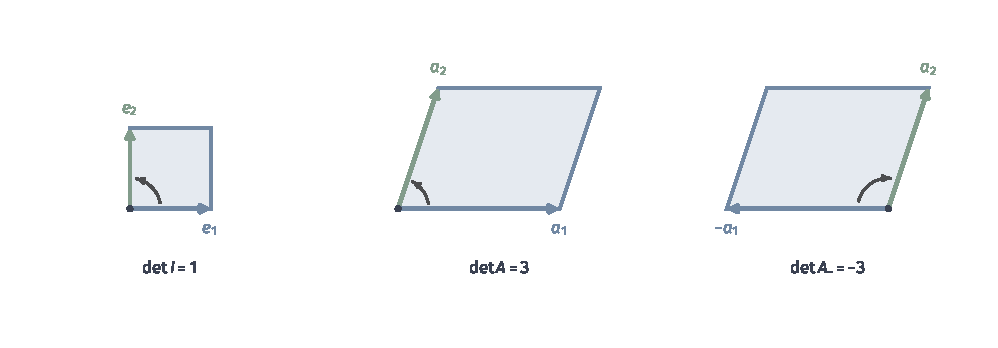
\includegraphics[width=169mm]{figures/00-shared/mathematical-preliminaries-upper/02-linear-spaces/matplotlib/ls-determinant-oriented-volume/ls-determinant-oriented-volume.pdf}
  \caption{行列式作为有向体积的缩放。左：单位正方形由$\bm e_1=(1,0)$、$\bm e_2=(0,1)$张成，面积为$1$。中：$\bm A=\bigl(\begin{smallmatrix}2&0.5\\0&1.5\end{smallmatrix}\bigr)$把它映成由$\bm A\bm e_1=(2,0)$、$\bm A\bm e_2=(0.5,1.5)$张成的平行四边形，有向面积为$2\cdot1.5-0.5\cdot0=3=\det\bm A>0$（保定向）。右：$\bm A$把$\bm e_1$反射到$(-2,0)$，有向面积为$-3$（反定向）。向量与数值均为解析教学例。}
  \label{fig:ls-determinant-oriented-volume}
\end{figure*}

\subsubsection{行列式的性质}

上一小节表明，行列式是各列张成的有向体积。下面的前两条性质就是有向体积的两条规则，其余性质由它们和排列公式推出。设$\bm A,\bm B$为$d$阶方阵。

\paragraph{对列的多线性}
三个矩阵只在同一列上不同、其余各列相同时，
\[
 \det\begin{bmatrix}\cdots&a\bm u+b\bm w&\cdots\end{bmatrix}
 =a\det\begin{bmatrix}\cdots&\bm u&\cdots\end{bmatrix}
 +b\det\begin{bmatrix}\cdots&\bm w&\cdots\end{bmatrix}.
\]

\paragraph{交替性}
交换两列，行列式变号；两列相同，行列式为零。前者是有向体积的规则，也已由排列公式验证。后者是因为交换两个相同的列不改变矩阵，行列式却要变号。

由多线性和交替性还能得到两个常用结论。第一，把某列的倍数加到另一列上，行列式不变：按多线性拆开后，多出的一项有两列相同，等于零。第二，某一列是其余各列的线性组合时，行列式为零：把这一列按组合展开，每一项都有两列相同。例如第二列是第一列的$2$倍时，
\[
 \det\begin{pmatrix}1&2\\2&4\end{pmatrix}=4-4=0.
\]

\paragraph{行变换与可逆性}
列上的这两条规则对行同样成立。排列公式的每一项从每行恰取一个元素，所以行列式对每一行也是线性的。交换第$i,k$两行，相当于把每个$\pi$与交换$i,k$的对换复合，逆序对数的奇偶随之改变，所以行列式变号。于是三种初等行变换对行列式的影响为：
\[
 \begin{aligned}
 &\text{交换两行：}&&\text{行列式变号；}\\
 &\text{某行乘以非零数}c\text{：}&&\text{行列式乘以}c\text{；}\\
 &\text{某行加上另一行的倍数：}&&\text{行列式不变。}
 \end{aligned}
\]

每一步消元都只使行列式乘以一个非零数，所以消元前后行列式是否为零不变。若某列找不到主元，阶梯形至少有一行全零；由对这一行的线性，行列式为零，矩阵也无法化为单位矩阵。若每列都找到主元，继续消元可以化为单位矩阵，而排列公式中$\det\bm I$只剩恒等排列一项，等于$1$，所以原矩阵的行列式非零，并且可以用第~\ref{sec:prelim-inverse-matrices}节的增广矩阵方法求逆。因此
\[
 \bm A\text{可逆}\iff\det\bm A\neq0.
\]

\paragraph{转置}
\[
 \det(\bm A^\top)=\det\bm A.
\]
$\bm A^\top$的排列公式为$\sum_\sigma\operatorname{sgn}(\sigma)\prod_j(\bm A^\top)_{j,\sigma(j)}=\sum_\sigma\operatorname{sgn}(\sigma)\prod_ja_{\sigma(j),j}$，这正是式~\eqref{eq:ls-det-column-form}。行列式对行和对列的性质因此完全对称。

\paragraph{数乘与加法}
\[
\begin{gathered}
\det(c\bm A)=c^d\det\bm A,\\
\det(\bm A+\bm B)\neq\det\bm A+\det\bm B\ (\text{一般}).
\end{gathered}
\]
数乘把$d$列各乘以$c$，由对每列的线性，提出$d$个$c$。行列式只对每一列分别线性，对整个矩阵却不是线性的。下面是一个反例。
\begin{example}[反例：行列式不保持加法]
\label{ex:ls-det-not-additive}
最简单的情形就足以说明问题。取$\bm A=\bm B=\bm I_2$，则$\det\bm A+\det\bm B=1+1=2$；而$\bm A+\bm B=2\bm I_2$，由上面的数乘公式，$\det(2\bm I_2)=2^2\det\bm I_2=4$。两者不等。原因在于两列同时加倍，体积要乘两次$2$。
\end{example}

\paragraph{乘法性}
\[
 \det(\bm A\bm B)=\det\bm A\,\det\bm B.
\]
从几何上看，接连作用两次，体积的放大倍数应当相乘。证明如下。固定$\bm A$，把$\det(\bm A\bm B)$看作$\bm B$的各列$\bm b_1,\ldots,\bm b_d$的函数
\[
 D(\bm b_1,\ldots,\bm b_d)=\det\begin{bmatrix}\bm A\bm b_1&\cdots&\bm A\bm b_d\end{bmatrix}=\det(\bm A\bm B).
\]
$\bm A\bm b_j$对$\bm b_j$线性，行列式对每列线性，所以$D$对每个$\bm b_j$线性；交换$\bm b_j,\bm b_k$就是交换$\bm A\bm B$的两列，$D$变号。由式~\eqref{eq:ls-det-volume}，
\[
 \det(\bm A\bm B)=D(\bm e_1,\ldots,\bm e_d)\det\bm B=\det\bm A\,\det\bm B.
\]
矩阵乘法不可交换，但$\det(\bm A\bm B)=\det(\bm B\bm A)$总成立，因为两边都等于$\det\bm A\,\det\bm B$。

\paragraph{三角矩阵的行列式}
\[
 \det\bm A=a_{1,1}a_{2,2}\cdots a_{d,d}\qquad(\bm A\text{为上三角或下三角矩阵}).
\]
设$\bm A$为上三角矩阵。若排列$\pi$不是恒等排列，必有某行$i$满足$\pi(i)<i$，因为$\sum_i(\pi(i)-i)=0$而各项不全为零。这一行取到主对角线下方的零元素，所以这一项为零，排列公式中只剩恒等排列一项。下三角时同理。例如
\[
 \det\begin{pmatrix}1&2&3\\0&4&5\\0&0&6\end{pmatrix}=1\cdot4\cdot6=24.
\]
特别地，$\det\operatorname{diag}(d_1,\ldots,d_d)=d_1\cdots d_d$。由乘法性，两个上三角矩阵乘积的行列式等于两者全部对角元之积，这与三角矩阵乘积的对角元逐个相乘一致。

结合行变换的规则，可以用消元计算行列式：先把方阵化为上三角矩阵，取对角元素的乘积，再补偿换行和倍乘的影响。例如
\[
 \det\begin{pmatrix}0&1&2\\1&2&1\\2&7&4\end{pmatrix}
 =-\det\begin{pmatrix}1&2&1\\0&1&2\\0&3&2\end{pmatrix}
 =-\det\begin{pmatrix}1&2&1\\0&1&2\\0&0&-4\end{pmatrix}=4.
\]
第一步交换前两行，并从第三行减去第一行的两倍；第二步从第三行减去第二行的三倍。交换行改变符号，两次加倍数不改变行列式。

\subsubsection{代数余子式与古典伴随}
\label{sec:ls-det-cofactor-adjugate}

排列公式有$d!$项。按某一行分组，可以把它化为$d$个$d-1$阶行列式。把这些低阶行列式排成矩阵，又能得到一个与$\bm A$相乘等于$(\det\bm A)\bm I_d$的矩阵。

\paragraph{按行（列）展开}
设$d\geq2$。删除第$i$行、第$j$列，得到的$(d-1)$阶子矩阵记为$\bm A^{(i,j)}$。定义\term{代数余子式}（cofactor）
\[
 C_{i,j}=(-1)^{i+j}\det\bm A^{(i,j)}.
\]
则对任一行$i$与任一列$j$，
\[
 \det\bm A=\sum_{j=1}^d a_{i,j}C_{i,j}=\sum_{i=1}^d a_{i,j}C_{i,j}.
\]
把排列公式按第$i$行所取的列分类，取第$j$列的各项之和正是$a_{i,j}C_{i,j}$；按列展开同理。下面沿第一行展开示例~\ref{ex:ls-det-three-by-three}中的矩阵，与排列公式的结果对照。
\begin{example}[沿第一行展开三阶行列式]
\label{ex:ls-det-cofactor-expansion}
仍取
\[
 \bm A=\begin{pmatrix}2&0&1\\1&3&0\\0&1&1\end{pmatrix}.
\]
第一行元素为$2,0,1$，对应代数余子式的符号$(-1)^{1+j}$依次为$+,-,+$。每个元素乘以删去它所在行、列后剩下的二阶行列式：
\[
 \begin{aligned}
 \det\bm A
 &=2\cdot\det\begin{pmatrix}3&0\\1&1\end{pmatrix}
 -0\cdot\det\begin{pmatrix}1&0\\0&1\end{pmatrix}
 +1\cdot\det\begin{pmatrix}1&3\\0&1\end{pmatrix}\\
 &=2\cdot3-0\cdot1+1\cdot1=7.
 \end{aligned}
\]
结果与示例~\ref{ex:ls-det-three-by-three}的排列展开一致。第一行的$0$使中间一项不必计算，所以按零较多的行或列展开最省事。
\end{example}

\paragraph{古典伴随恒等式}
把全部代数余子式排成矩阵$\bm C$，其转置$\operatorname{adj}(\bm A)=\bm C^\top$称为\term{古典伴随}（classical adjugate）。
\begin{theorem}[古典伴随恒等式]
\label{thm:ls-adjugate-identity}
对任意$d$阶方阵$\bm A$，
\[
 \bm A\,\operatorname{adj}(\bm A)
 =\operatorname{adj}(\bm A)\,\bm A
 =(\det\bm A)\,\bm I_d.
\]
\end{theorem}
\begin{proof}
乘积$\bm A\bm C^\top$的$(i,k)$元素为$\sum_j a_{i,j}C_{k,j}$。当$i=k$时，这正是沿第$i$行展开的$\det\bm A$。当$i\neq k$时，$C_{k,j}$不涉及第$k$行的元素，所以这个和是把第$k$行换成第$i$行后所得矩阵沿第$k$行的展开；新矩阵有两行相同，行列式为零。于是$\bm A\bm C^\top=(\det\bm A)\bm I_d$。按列展开，同样得到$\bm C^\top\bm A=(\det\bm A)\bm I_d$。
\end{proof}
二阶时
\[
 \operatorname{adj}\begin{pmatrix}a&b\\c&d\end{pmatrix}=\begin{pmatrix}d&-b\\-c&a\end{pmatrix},
\]
恒等式两边除以$ad-bc$，就是第~\ref{sec:prelim-inverse-matrices}节的二阶求逆公式。

古典伴随是由余子式得到的代数构造，与第~\ref{sec:ls-adjoints}节由内积定义的伴随不是同一个对象。高阶时展开余子式的代价是阶乘级的，所以这个恒等式主要用作证明工具。下面用它证明方阵的单侧逆即逆；后文还用它给出线性方程的可逆判据（第~\ref{sec:ls-determinant-invertibility}节），并证明Cayley--Hamilton定理（第~\ref{sec:ls-characteristic-polynomial}节）。

\paragraph{方阵的单侧逆即逆}
\phantomsection
\label{sec:ls-square-one-sided-inverse}
第~\ref{sec:prelim-inverse-matrices}节定义逆矩阵时，要求两侧乘积都等于单位矩阵。对方阵，一侧就够了。
\begin{theorem}[方阵的单侧逆即逆]
\label{thm:ls-square-one-sided-inverse}
设$\bm A,\bm B$为$n$阶方阵。若$\bm B\bm A=\bm I_n$或$\bm A\bm B=\bm I_n$，则$\bm A$可逆且$\bm B=\bm A^{-1}$。
\end{theorem}
\begin{proof}
由乘法性，两种情形都有$\det\bm A\det\bm B=\det\bm I_n=1$，所以$\det\bm A\neq0$。令$\bm C=\operatorname{adj}(\bm A)/\det\bm A$，由古典伴随恒等式，$\bm A\bm C=\bm C\bm A=\bm I_n$，所以$\bm A$可逆，且$\bm C=\bm A^{-1}$。若$\bm B\bm A=\bm I_n$，则$\bm B=\bm B(\bm A\bm C)=(\bm B\bm A)\bm C=\bm C$；若$\bm A\bm B=\bm I_n$，则$\bm B=(\bm C\bm A)\bm B=\bm C(\bm A\bm B)=\bm C$。
\end{proof}
所以检验方阵的逆，只需验证一侧的乘积。矩形矩阵则不同：左逆与右逆可以只存在一个，也可以不唯一（示例~\ref{ex:ls-left-inverse-not-unique}）。

\subsection{迹}
\label{sec:prelim-matrix-trace}

行列式要用到方阵的全部元素。迹只看主对角线：$n$阶方阵的\term{迹}（trace）是主对角元素之和，
\[
 \operatorname{tr}(\bm A)=\sum_{i=1}^n A_{i,i}.
\]
例如
\[
 \operatorname{tr}\begin{pmatrix}1&2\\3&4\end{pmatrix}=1+4=5,
\]
而这个矩阵全部元素之和是$10$。迹只对方阵定义，只累加对角元。

\subsubsection{迹的性质}
\phantomsection
\label{sec:ls-matrix-contractions}

迹是有限和，前两条性质可以直接看出；第三条循环性是迹最常用的性质。

\paragraph{线性}
\[
 \operatorname{tr}(a\bm A+b\bm B)=a\operatorname{tr}(\bm A)+b\operatorname{tr}(\bm B),
\]
这是有限和的线性。

\paragraph{转置不变}
\[
 \operatorname{tr}(\bm A^\top)=\operatorname{tr}(\bm A),
\]
因为转置不改变对角元。

\paragraph{循环性}
对$\bm A\in\mathbb R^{m\times n}$、$\bm B\in\mathbb R^{n\times m}$，
\begin{equation}
 \operatorname{tr}(\bm A\bm B)
 =\sum_{i=1}^m\sum_{j=1}^n A_{i,j}B_{j,i}
 =\operatorname{tr}(\bm B\bm A).
 \label{eq:linear-algebra-trace-cyclic}
\end{equation}
两个双重和只是求和次序不同。$\bm A\bm B$与$\bm B\bm A$可以是不同阶的方阵；相等的是它们的迹，不是矩阵本身。下面的例子说明这一点。
\begin{example}[不同阶乘积的迹相等]
\label{ex:ls-trace-cyclic-different-sizes}
取行向量$\bm A=\left[\begin{smallmatrix}1&2&3\end{smallmatrix}\right]\in\mathbb R^{1\times3}$与列向量$\bm B=(1,0,2)^\top\in\mathbb R^{3\times1}$。按“行乘列”的次序，$\bm A\bm B=1\cdot1+2\cdot0+3\cdot2=7$是$1\times1$矩阵；按“列乘行”的次序，
\[
 \bm B\bm A=\begin{bmatrix}1&2&3\\0&0&0\\2&4&6\end{bmatrix}
\]
是$3\times3$矩阵，对角元为$1,0,6$。两个乘积连阶数都不同，迹却相等：$\operatorname{tr}(\bm A\bm B)=7=1+0+6=\operatorname{tr}(\bm B\bm A)$。$\bm B\bm A$的对角元$A_{1,j}B_{j,1}$恰好是内积$\bm A\bm B$中的三项。
\end{example}

三个因子时，循环性只允许把因子整体循环移动：
\[
 \operatorname{tr}(\bm A\bm B\bm C)=\operatorname{tr}(\bm B\bm C\bm A)=\operatorname{tr}(\bm C\bm A\bm B).
\]
第一个等号把$\bm A$与$\bm B\bm C$看作两个因子，使用式~\eqref{eq:linear-algebra-trace-cyclic}；第二个等号把$\bm A\bm B$与$\bm C$看作两个因子。任意交换相邻因子则可能改变迹，下面是一个反例。
\begin{example}[反例：交换相邻因子会改变迹]
\label{ex:ls-trace-adjacent-swap}
取
\[
 \bm A=\begin{pmatrix}1&0\\0&0\end{pmatrix},\quad
 \bm B=\begin{pmatrix}0&0\\1&0\end{pmatrix},\quad
 \bm C=\begin{pmatrix}0&1\\0&0\end{pmatrix}.
\]
其中$\bm A,\bm B$就是示例~\ref{ex:ls-zero-product-nonzero-factors}中的两个矩阵，$\bm A\bm B=\bm0$，所以$\bm A\bm B\bm C=\bm0$。把$\bm B$与$\bm C$对调：$\bm C$的非零元在第一行，$\bm A$保留第一行，故$\bm A\bm C=\bm C$，从而
\[
 \bm A\bm C\bm B=\begin{pmatrix}0&1\\0&0\end{pmatrix}\begin{pmatrix}0&0\\1&0\end{pmatrix}=\begin{pmatrix}1&0\\0&0\end{pmatrix}.
\]
于是$\operatorname{tr}(\bm A\bm B\bm C)=0$，而$\operatorname{tr}(\bm A\bm C\bm B)=1$。$\bm A\bm C\bm B$不是$\bm A\bm B\bm C$的循环移动，迹可以不同。
\end{example}

\subsection{矩阵的元素内积}

行列式和迹都只对方阵定义，只用到一个矩阵。比较两个同形矩阵时，可以像向量内积那样，把全部对应元素配对。

\subsubsection{Frobenius内积}

把同形矩阵的$mn$个元素看作$mn$个坐标，照搬欧氏内积，就得到\term{Frobenius内积}：对$\bm A,\bm B\in\mathbb R^{m\times n}$，
\[
 \langle\bm A,\bm B\rangle_{\mathrm F}=\sum_{i=1}^m\sum_{j=1}^na_{i,j}b_{i,j}.
\]
它把对应元素逐项相乘后全部相加，也就是$\bm A\odot\bm B$全部元素之和。下面沿用逐项乘积一例中的两个矩阵。
\begin{example}[Frobenius内积的计算]
\label{ex:ls-frobenius-inner-product}
对
\[
 \bm A=\begin{pmatrix}1&2\\3&4\end{pmatrix},\quad
 \bm B=\begin{pmatrix}0&1\\1&0\end{pmatrix},
\]
按位置$(1,1),(1,2),(2,1),(2,2)$依次配对相乘再相加：
\[
 \langle\bm A,\bm B\rangle_{\mathrm F}=1\cdot0+2\cdot1+3\cdot1+4\cdot0=5.
\]
四个乘积正是示例~\ref{ex:ls-hadamard-vs-matrix-product}中$\bm A\odot\bm B$的四个元素$0,2,3,0$，所以Frobenius内积就是逐项乘积的元素之和。
\end{example}

\paragraph{Frobenius内积的迹表示}
Frobenius内积可以用迹写出：
\[
 \begin{gathered}
 \langle\bm A,\bm B\rangle_{\mathrm F}=\operatorname{tr}(\bm A^\top\bm B),\\
 \lVert\bm A\rVert_{\mathrm F}^2=\operatorname{tr}(\bm A^\top\bm A).
 \end{gathered}
\]
$\bm A^\top\bm B$的第$j$个对角元为$\sum_i A_{i,j}B_{i,j}$，再对$j$求和，恰好遍历所有位置。第二式中的$\lVert\bm A\rVert_{\mathrm F}$就是下面定义的Frobenius范数。反过来，计算$\operatorname{tr}(\bm A\bm B)$时也不必先求出乘积：只需计算$\sum_{i,j}A_{i,j}B_{j,i}$，代价为$mn$次乘法，而求出整个$\bm A\bm B$需要$m^2n$次。

\subsubsection{Frobenius范数}
\label{sec:ls-frobenius-norm}

由Frobenius内积可以定义矩阵的大小。把矩阵当作一张数表，定义Frobenius范数
\[
 \lVert\bm A\rVert_{\mathrm F}=\sqrt{\langle\bm A,\bm A\rangle_{\mathrm F}}=\left(\sum_{i,j}a_{i,j}^2\right)^{1/2}.
\]
例如
\[
 \left\lVert\begin{pmatrix}1&2\\3&4\end{pmatrix}\right\rVert_{\mathrm F}=\sqrt{1+4+9+16}=\sqrt{30}.
\]
它就是把$mn$个元素排成一列以后的$2$范数，其范数性质在第~\ref{sec:ls-normed-space-definition}节由Minkowski不等式统一验证。

Frobenius范数也可以从矩阵的作用来理解。由$\bm A\bm e_j=\bm A_{:,j}$，
\[
 \lVert\bm A\rVert_{\mathrm F}^2=\sum_j\lVert\bm A_{:,j}\rVert_2^2=\sum_j\lVert\bm A\bm e_j\rVert_2^2,
\]
即全部标准坐标向量输入后，输出长度的平方和。它不是某一个最坏输入的放大倍数；后者是另一种矩阵范数，在第~\ref{sec:ls-matrix-norms}节讨论。

数据按组划分时，还可以先在组内汇总、再汇总各组，得到混合范数。例如以行为组，$\lVert\bm A\rVert_{p,q}=(\sum_i\lVert\bm A_{i,:}\rVert_p^q)^{1/q}$：内层的$p$范数衡量每一行的大小，外层的$q$范数汇总各行。

% 第1章第4节：张量的表示（多维数组、轴、阶、形状、切片）；张量的重排（轴置换、形状重整与向量化及重排的性质）、张量积及其性质、Kronecker积及其性质、指标缩约及其性质。各种乘积的形状汇总见本章小结。

\section{张量}
\label{sec:ls-tensors-objects}

一批图像要记录样本、通道和两个像素坐标，一批文本要记录样本、位置和特征维度。定位其中一个数需要三个甚至更多的索引，一张矩阵装不下。本节先给出多维数组的记法，再按对轴的作用讨论三类运算：重排只改变元素所在的位置；张量积与Kronecker积把几个数组组合成轴更多的数组；缩约沿指定的轴求和，把数组汇总成轴更少的数组。每类运算之后整理它的性质。最后会看到，前两节的内积、矩阵乘法与迹都是缩约。

\subsection{张量的表示}
\label{sec:ls-tensor-representation}

向量用一个索引定位一个数，矩阵用两个。一个量由更多路索引共同决定时，就需要更多索引。机器学习中常把这样的多索引数值数组称为\term{张量}（tensor）。

数学中的“张量”还有不依赖坐标的定义，例如多线性映射或张量积空间的元素；本节只采用坐标数组的口径，把张量当作一张多索引的数表。数组与多线性映射的联系，在第~\ref{sec:ls-multilinear-maps}节选定基以后说明。
\begin{definition}[多维数值数组]
\label{def:linear-algebra-multidimensional-array}
给定正整数$n_1,\ldots,n_k$，形状为$n_1\times\cdots\times n_k$的数值数组，是从$\{1,\ldots,n_1\}\times\cdots\times\{1,\ldots,n_k\}$到$\mathbb R$的映射。第$j$个索引称为第$j$个\term{轴}（axis），轴数$k$称为数组的\term{阶}（order）。
\end{definition}
按这一定义，向量是一阶数组，矩阵是二阶数组；并约定单个标量是零阶数组。阶是索引的个数，形状记录各轴的长度。轴的长度再大也不改变阶：$\mathbb R^{100}$中的向量仍是一阶数组。

例如$\bm X\in\mathbb R^{b\times\ell\times d}$可以记录$b$个样本、每个样本$\ell$个位置、每个位置$d$个特征，元素$x_{i,j,k}$由三个索引共同定位。固定一部分索引，得到切片：$\bm X_{i,:,:}$保留第$i$个样本，是一个$\ell\times d$矩阵；$\bm X_{i,j,:}$再固定位置，是一个$d$维向量。图~\ref{fig:ls-scalar-vector-matrix-tensor}按“定位一个数需要几个索引”并排比较四类数组。
\begin{figure}[!htb]
  \centering
  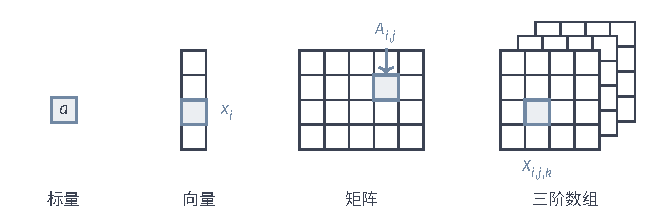
\includegraphics[width=112mm]{figures/00-shared/mathematical-preliminaries-upper/02-linear-spaces/tikz/comprehension-additions/scalar-vector-matrix-tensor.pdf}
  \caption{标量、向量、矩阵与三阶数组的区别。每个面板用蓝色标出一个数：标量本身就是这个数，向量用一个索引$i$定位，矩阵用行列两个索引$i,j$定位，三阶数组再加一个索引$k$选择切片。索引个数称为阶，各轴长度组成形状。}
  \label{fig:ls-scalar-vector-matrix-tensor}
\end{figure}

两个同形数组按位置逐项相加和数乘，规则与向量、矩阵相同。两个数组相加，仍要求形状相同、对应轴的含义相同。所以使用多维数组时，要先说清每条轴记录什么。同一个$b\times\ell\times d$数组，若把第二、三轴的含义弄反，后面的每一次汇总都会汇总到错误的轴上。

\subsection{张量的重排}
\label{sec:ls-tensor-operations}

有了记法，先看第一类运算：重排。轴置换与形状重整只改变元素记录在哪条轴、哪个位置上，既不改变数值，也不求和。下面先讨论这两种重排，再整理它们共同的性质。

\subsubsection{轴置换}
\label{sec:ls-tensor-reshaping}
\phantomsection
\label{sec:linear-algebra-tensors-structured-operations}

\term{维度重排}（permutation of axes）也称轴置换，它按给定顺序调换轴的位置，每个元素跟着自己的索引移动。计算时先写出新旧索引的对应，再按对应搬运元素。例如把$\bm X\in\mathbb R^{b\times\ell\times d}$的第二、三轴互换，得到$\bm Y\in\mathbb R^{b\times d\times\ell}$，
\[
 y_{i,k,j}=x_{i,j,k}.
\]
第一轴保持原位，每个样本的切片被转置：$\bm Y_{i,:,:}=(\bm X_{i,:,:})^\top$。下面取一个具体的小数组。
\begin{example}[交换后两条轴]
\label{ex:ls-axis-swap}
取$b=1$、$\ell=2$、$d=3$，这时数组只有一个样本切片
\[
 \bm X_{1,:,:}=\begin{bmatrix}1&2&3\\4&5&6\end{bmatrix}.
\]
按$y_{1,k,j}=x_{1,j,k}$逐个搬运元素。例如原来位于第$2$个位置、第$3$个特征的$6$，搬到$y_{1,3,2}$。全部搬完，得到
\[
 \bm Y_{1,:,:}=\begin{bmatrix}1&4\\2&5\\3&6\end{bmatrix}.
\]
新数组$\bm Y\in\mathbb R^{1\times3\times2}$的样本切片正是原切片的转置，数值一个也没有改变。
\end{example}
只有两条轴时，唯一不平凡的轴置换就是矩阵的转置。轴的含义跟着轴走，不因位置改变而改变：$\bm Y$的第二轴仍是特征，第三轴仍是位置。

\subsubsection{形状重整与向量化}

\term{形状重整}（reshape）分两步：先按指定的遍历顺序把全部元素读成一个数列，再把这个数列按同样的顺序装入另一种形状。它只要求元素总数不变。形状重整与转置都能把$2\times3$矩阵变成$3\times2$矩阵，但结果不同。
\begin{example}[按行重整与转置的区别]
\label{ex:ls-reshape-vs-transpose}
把
\[
 \bm A=\begin{bmatrix}1&2&3\\4&5&6\end{bmatrix}
\]
按行重整为$3\times2$数组：先按行读出数列$1,2,3,4,5,6$，再按行依次装入，得到下面的$\bm R$。作为对照，同时写出转置$\bm A^\top$：
\[
\begin{gathered}
\bm R=\begin{bmatrix}1&2\\3&4\\5&6\end{bmatrix},\\
\text{而}\qquad
 \bm A^\top=\begin{bmatrix}1&4\\2&5\\3&6\end{bmatrix}.
\end{gathered}
\]
$\bm R$与$\bm A^\top$形状相同、所含的数相同，排列却不同。$\bm A^\top$的第一列是$\bm A$原来的第一行$1,2,3$，$\bm R$的第一列却是$1,3,5$，把原来的行拆散了。
\end{example}
所以描述一次重整，除了目标形状，还要给出遍历顺序；形状对了，也不说明完成了轴交换。图~\ref{fig:vol1-add-linear-transpose-reshape}把两种结果并排放置。
\begin{figure}[!htb]
  \centering
  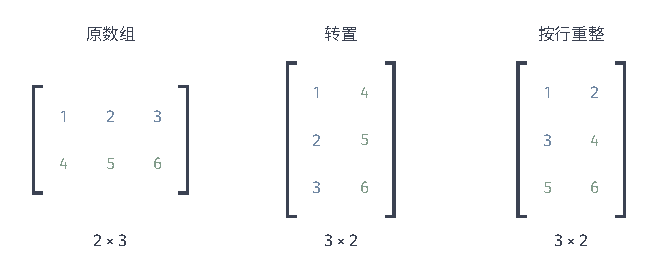
\includegraphics[width=112mm]{figures/00-shared/mathematical-preliminaries-upper/02-linear-spaces/tikz/comprehension-additions/linear-transpose-reshape.pdf}
  \caption{轴交换与按行重整。原数组两行为$(1,2,3)$与$(4,5,6)$；中图转置后两列分别保留原来的两行，右图则把按行读取的数列$1,2,3,4,5,6$依次装入$3\times2$数组。数字及其排列与正文示例相同。}
  \label{fig:vol1-add-linear-transpose-reshape}
\end{figure}

最常用的一种形状重整，是把矩阵按列堆叠成一个长列向量，称为\term{向量化}（vectorization）：
\[
 \operatorname{vec}(\bm A)=(a_{1,1},\ldots,a_{m,1},a_{1,2},\ldots,a_{m,2},\ldots,a_{1,n},\ldots,a_{m,n})^\top.
\]
$m\times n$矩阵的元素$a_{i,j}$位于第$i+(j-1)m$个位置。例如上面的$\bm A$给出$\operatorname{vec}(\bm A)=(1,4,2,5,3,6)^\top$，其中$a_{2,3}=6$位于第$2+(3-1)\cdot2=6$个位置。

多维数组也可以重整成矩阵，称为矩阵展开（unfolding）：把一部分轴合并成行索引，其余轴合并成列索引。例如把$\bm X\in\mathbb R^{b\times\ell\times d}$的前两轴合并为行，得到$b\ell\times d$矩阵，每行是一个样本在一个位置上的特征。合并哪些轴，决定了展开结果的形状，也决定了后续乘积汇总哪条轴。

\subsubsection{重排的性质}

固定轴的顺序和遍历规则以后，重排有三条性质：它不丢失信息，与逐项运算可交换，但一般的形状重整与矩阵乘法不相容。

\paragraph{可逆性}
目标形状与遍历顺序固定后，轴置换、形状重整与向量化都把一个数组一一对应到另一个数组，逆操作可以恢复原数组：
\[
 (\bm A^\top)^\top=\bm A,\qquad
 \operatorname{vec}^{-1}\bigl(\operatorname{vec}(\bm A)\bigr)=\bm A.
\]
这里$\operatorname{vec}^{-1}$把长度为$mn$的向量依次每$m$个一列装回$m\times n$矩阵。一般的轴置换按逆置换换回，形状重整按原顺序装回。所以重排保留全部信息。

\paragraph{线性}
\[
 \operatorname{vec}(a\bm A+b\bm B)=a\operatorname{vec}(\bm A)+b\operatorname{vec}(\bm B).
\]
轴置换与形状重整同样满足这一性质：它们只搬动元素，逐项的加法与数乘搬到新位置后不变。

\paragraph{与矩阵乘法的关系}
转置与乘法有整齐的规则
\[
 (\bm A\bm B)^\top=\bm B^\top\bm A^\top,
\]
一般的形状重整却没有。重整以后，每一行、每一列汇集的元素都变了，依赖行列结构的乘积、迹与行列式一般随之改变。下面的反例把示例~\ref{ex:ls-reshape-vs-transpose}中的$\bm R$误当作$\bm A^\top$使用。
\begin{example}[反例：重整不能代替转置]
\label{ex:ls-reshape-breaks-product}
仍取$\bm A$与按行重整得到的$\bm R$，
\[
 \bm A=\begin{bmatrix}1&2&3\\4&5&6\end{bmatrix},\qquad
 \bm R=\begin{bmatrix}1&2\\3&4\\5&6\end{bmatrix}.
\]
示例~\ref{ex:ls-gram-product-symmetric}已经算出
\[
 \bm A\bm A^\top=\begin{bmatrix}14&32\\32&77\end{bmatrix};
\]
而
\[
 \bm A\bm R=\begin{bmatrix}1+6+15&2+8+18\\4+15+30&8+20+36\end{bmatrix}=\begin{bmatrix}22&28\\49&64\end{bmatrix}.
\]
$\bm R$与$\bm A^\top$形状相同、所含的数相同，两个乘积却完全不同：$\bm A\bm R$不对称，迹也从$14+77=91$变成$22+64=86$。原因是乘积按行列配对元素，而重整改变了哪些元素同在一列。
\end{example}
把存储格式的改变误当成计算上的变换，是使用重整时最常见的错误。

\subsection{张量积}
\label{sec:ls-tensor-products}
\phantomsection
\label{sec:linear-algebra-joint-operations}

第二类运算把几个数组组合起来。最基本的情形是两个向量：把它们的全部两两乘积排成一个数组，就是张量积。

设$\bm x\in\mathbb R^m$、$\bm y\in\mathbb R^n$，\term{张量积}（tensor product）$\bm x\otimes\bm y$是$m\times n$数组，
\[
 (\bm x\otimes\bm y)_{i,j}=x_i y_j.
\]
写成矩阵，$\bm x\otimes\bm y=\bm x\bm y^\top$，正是分块乘法式~\eqref{eq:ls-product-outer-sum}中“一列乘一行”的矩阵。每个因子各占结果的一条轴，下面把这条轴称为该因子的槽位。三个向量的张量积$(\bm x\otimes\bm y\otimes\bm z)_{i,j,k}=x_i y_j z_k$有三个槽位，更多因子按同样规则逐槽位相乘。下面计算两个二维向量的张量积。
\begin{example}[两个二维向量的张量积]
\label{ex:ls-tensor-product-two-vectors}
取$\bm x=(1,2)^\top$与$\bm y=(3,-1)^\top$，把$x_i$与$y_j$的乘积填在位置$(i,j)$：
\[
 \bm x\otimes\bm y=\begin{pmatrix}1\cdot3&1\cdot(-1)\\2\cdot3&2\cdot(-1)\end{pmatrix}=\begin{pmatrix}3&-1\\6&-2\end{pmatrix}.
\]
第二行$(6,-2)$恰是第一行$(3,-1)$的$2$倍。一般地，第$i$行是$x_i\bm y^\top$，每一行都是$\bm y^\top$的倍数；同理，每一列都是$\bm x$的倍数。
\end{example}
两个因子的长度不必相同。图~\ref{fig:ls-tensor-product-slots}取$\bm u=(1,2)^\top$与三维的$\bm v=(3,-1,2)^\top$：第一个因子占行轴，第二个因子占列轴，结果的第$i$行是$u_i\bm v^\top$，第$j$列是$v_j\bm u$。
\begin{figure}[htbp]
  \centering
  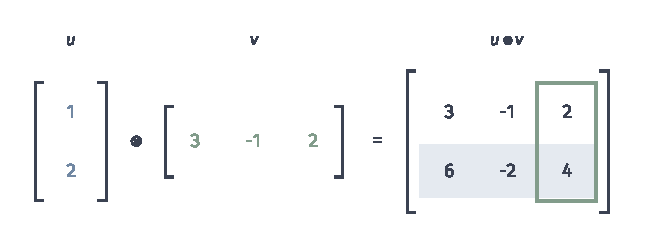
\includegraphics[width=112mm]{figures/00-shared/mathematical-preliminaries-upper/02-linear-spaces/matplotlib/ls-tensor-product-slots/ls-tensor-product-slots.pdf}
  \caption{张量积的两个槽位。左：$\bm u=(1,2)^\top\in\mathbb R^2$竖排，$\bm v=(3,-1,2)^\top\in\mathbb R^3$横排。右：$\bm u\otimes\bm v$是$2\times3$数组，行由$u_i$标记、列由$v_j$标记，位置$(i,j)$的元素为$u_iv_j$。蓝色实线框标出第2行$(6,-2,4)=u_2\bm v^\top$，绿色虚线框标出第3列$(2,4)^\top=v_3\bm u$。数值由定义直接相乘得到，是教学构造。}
  \label{fig:ls-tensor-product-slots}
\end{figure}

同样的配对规则适用于任意有限数组。设$\bm A$有$k$条轴、形状为$n_1\times\cdots\times n_k$，$\bm B$有$\ell$条轴、形状为$m_1\times\cdots\times m_\ell$。它们的数组张量积保留两组索引：
\[
 (\bm A\otimes\bm B)_{i_1,\ldots,i_k,j_1,\ldots,j_\ell}
 =a_{i_1,\ldots,i_k}b_{j_1,\ldots,j_\ell}.
\]
输出有$k+\ell$条轴，长度依次与输入的各轴相同；这里没有对任何索引求和。交换两个输入，会同时交换两组轴的次序。实数乘积$ab=ba$，并不意味着$\bm A\otimes\bm B$与$\bm B\otimes\bm A$相同。

形如$\bm x\otimes\bm y$的数组称为\term{简单张量}（simple tensor）。由示例~\ref{ex:ls-tensor-product-two-vectors}，简单张量的各行都是同一个向量的倍数。所以并非每个二阶数组都是简单张量，下面是一个反例。
\begin{example}[反例：单位矩阵不是简单张量]
\label{ex:ls-identity-not-simple}
$\bm I_2$的两行为$(1,0)$与$(0,1)$。假设$\bm I_2=\bm x\otimes\bm y$，则两行分别是$x_1\bm y^\top$与$x_2\bm y^\top$。两行都非零，所以$x_1,x_2\neq0$，两行都是$\bm y^\top$的非零倍数，从而彼此成比例。但$(1,0)$与$(0,1)$不成比例，矛盾。所以$\bm I_2$不能写成任何$\bm x\otimes\bm y$，它不是简单张量。
\end{example}
不过，每个$m\times n$数组$\bm T$都是简单张量的和：
\[
 \bm T=\sum_{i,j}t_{i,j}\,\bm e_i\otimes\bm f_j,
\]
其中$\bm e_i$、$\bm f_j$分别是$\mathbb R^m$与$\mathbb R^n$的标准坐标向量，$\bm e_i\otimes\bm f_j$只在位置$(i,j)$为$1$。

张量积的用处，是把同时依赖两组输入的计算，化为对单个数组的线性计算。设实值函数$B(\bm x,\bm y)$对$\bm x$、$\bm y$分别保持线性组合，这样的函数称为双线性的。把$\bm x=\sum_ix_i\bm e_i$、$\bm y=\sum_jy_j\bm f_j$代入，按两次线性展开，
\[
 B(\bm x,\bm y)=\sum_{i,j}x_iy_j\,B(\bm e_i,\bm f_j)=\sum_{i,j}g_{i,j}(\bm x\otimes\bm y)_{i,j}
 =\langle\bm G,\bm x\otimes\bm y\rangle_{\mathrm F},
\]
其中$g_{i,j}=B(\bm e_i,\bm f_j)$。所以双线性函数由一张固定的系数表$\bm G$决定，并且它作为$\bm x\otimes\bm y$的函数是线性的。以欧氏内积$B(\bm x,\bm y)=\bm x^\top\bm y$（$m=n$）为例，$g_{i,j}=\langle\bm e_i,\bm e_j\rangle$，即$\bm G=\bm I$，这时计算就是把$\bm x\otimes\bm y$的对角元加起来。

二阶张量与矩阵是同一组数的两种看法：张量强调每个槽位来自哪一组输入，矩阵强调行与列在乘法中的角色。

\subsubsection{张量积的性质}
\label{sec:ls-tensor-product-properties}

张量积的每个元素都是各因子元素的乘积，下面的性质都从这个元素公式逐槽位验证。

\paragraph{对每个因子线性}
\[
 \begin{gathered}
(a\bm x)\otimes\bm y=\bm x\otimes(a\bm y)=a(\bm x\otimes\bm y),\\
(\bm x+\bm x')\otimes\bm y=\bm x\otimes\bm y+\bm x'\otimes\bm y,\\
\bm x\otimes(\bm y+\bm y')=\bm x\otimes\bm y+\bm x\otimes\bm y'.
 \end{gathered}
\]
每个元素$x_iy_j$对$x_i$和$y_j$分别线性，逐项验证即得。

\paragraph{结合律}
\[
 (\bm x\otimes\bm y)\otimes\bm z=\bm x\otimes(\bm y\otimes\bm z),
\]
两边的$(i,j,k)$元素都是$x_iy_jz_k$。

\paragraph{交换槽位是转置}
\[
 \bm y\otimes\bm x=(\bm x\otimes\bm y)^\top,
\]
因为$\bm x\otimes\bm y$的$(i,j)$元素$x_iy_j$也是$\bm y\otimes\bm x$的$(j,i)$元素。所以一般$\bm x\otimes\bm y\neq\bm y\otimes\bm x$，两者相差一次轴置换。

\paragraph{Frobenius配对与范数分离}
\[
 \begin{gathered}
\langle\bm x\otimes\bm y,\bm x'\otimes\bm y'\rangle_{\mathrm F}
 =\langle\bm x,\bm x'\rangle\langle\bm y,\bm y'\rangle,\\
\lVert\bm x\otimes\bm y\rVert_{\mathrm F}=\lVert\bm x\rVert_2\,\lVert\bm y\rVert_2.
 \end{gathered}
\]
第一式来自$\sum_{i,j}x_iy_jx'_iy'_j=(\sum_ix_ix'_i)(\sum_jy_jy'_j)$；在第一式中取$\bm x'=\bm x$、$\bm y'=\bm y$，再开平方，得到第二式。下面在示例~\ref{ex:ls-tensor-product-two-vectors}的数组上核对第二式。
\begin{example}[张量积范数的数值核对]
\label{ex:ls-tensor-product-norm-check}
仍取$\bm x=(1,2)^\top$与$\bm y=(3,-1)^\top$，它们的张量积为
\[
 \bm x\otimes\bm y=\begin{pmatrix}3&-1\\6&-2\end{pmatrix}.
\]
按公式右端，只需两个向量各自的长度：$\lVert\bm x\rVert_2=\sqrt5$，$\lVert\bm y\rVert_2=\sqrt{10}$，乘积为$\sqrt5\cdot\sqrt{10}=\sqrt{50}=5\sqrt2$。直接对四个元素求Frobenius范数，
\[
 \lVert\bm x\otimes\bm y\rVert_{\mathrm F}=\sqrt{3^2+(-1)^2+6^2+(-2)^2}=\sqrt{50},
\]
两种算法一致。
\end{example}

\paragraph{与行列式的联系}
把张量积反对称化，得到$\bm x\otimes\bm y-\bm y\otimes\bm x$。它的$(i,j)$元素为
\[
 x_iy_j-x_jy_i=\det\begin{pmatrix}x_i&y_i\\x_j&y_j\end{pmatrix},
\]
即把$\bm x,\bm y$投影到第$i,j$两个坐标构成的平面后张成的有向面积（第~\ref{sec:ls-exterior-determinants}节）。交换$\bm x,\bm y$时，每个元素都变号。

\subsection{Kronecker积}

两个矩阵分别作用在两条轴上时，可以把联合作用写成一张大矩阵，这就是Kronecker积。对$\bm A\in\mathbb R^{m\times n}$、$\bm B\in\mathbb R^{p\times q}$，定义
\begin{equation}
 \bm A\otimes\bm B
 =\begin{bmatrix}
  A_{1,1}\bm B&\cdots&A_{1,n}\bm B\\
  \vdots&\ddots&\vdots\\
  A_{m,1}\bm B&\cdots&A_{m,n}\bm B
 \end{bmatrix}\in\mathbb R^{mp\times nq}.
 \label{eq:linear-algebra-kronecker-product}
\end{equation}
计算时，把$\bm A$的每个元素$A_{i,j}$替换成块$A_{i,j}\bm B$。下面计算一个二阶的例子。
\begin{example}[两个二阶矩阵的Kronecker积]
\label{ex:ls-kronecker-two-by-two}
取
\[
 \bm A=\begin{bmatrix}1&2\\3&4\end{bmatrix},\quad
 \bm B=\begin{bmatrix}0&1\\1&0\end{bmatrix},
\]
把$\bm A$的四个元素分别换成块$1\cdot\bm B$、$2\cdot\bm B$、$3\cdot\bm B$、$4\cdot\bm B$：
\[
 \bm A\otimes\bm B
 =\begin{bmatrix}
  1\cdot\bm B&2\cdot\bm B\\
  3\cdot\bm B&4\cdot\bm B
 \end{bmatrix}
 =\begin{bmatrix}0&1&0&2\\1&0&2&0\\0&3&0&4\\3&0&4&0\end{bmatrix}.
\]
结果是$4\times4$矩阵。每个$2\times2$块都是$\bm B$乘以$\bm A$的一个元素，块的排列照搬$\bm A$中元素的位置：$\bm A$的形状与元素决定块怎样排、各乘多少，$\bm B$决定每块内部的样子。
\end{example}
图~\ref{fig:ls-kronecker-block-structure}用另一组数展示这种逐元素替换得到的分块结构。
\begin{figure}[htbp]
  \centering
  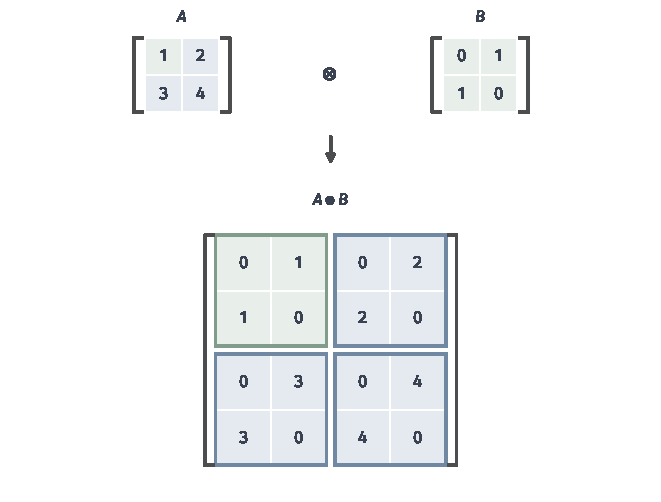
\includegraphics[width=112mm]{figures/00-shared/mathematical-preliminaries-upper/02-linear-spaces/matplotlib/ls-kronecker-block-structure/ls-kronecker-block-structure.pdf}
  \caption{Kronecker积的分块结构。上：$\bm A=\bigl(\begin{smallmatrix}1&2\\3&4\end{smallmatrix}\bigr)$、$\bm B=\bigl(\begin{smallmatrix}10&20\\30&40\end{smallmatrix}\bigr)$。下：$\bm A\otimes\bm B$是把$\bm A$的每个元素替换为该元素乘$\bm B$得到的$4\times4$分块矩阵，块边界用白线强调。数值由定义直接计算，是教学例。}
  \label{fig:ls-kronecker-block-structure}
\end{figure}

Kronecker积与张量积用同一个记号$\otimes$，两者记录的是同一组数，只是排法不同。两个列向量按式~\eqref{eq:linear-algebra-kronecker-product}相乘，得到$mn$维长向量$(x_1\bm y^\top,\ldots,x_m\bm y^\top)^\top$，它正是把$m\times n$数组$\bm x\otimes\bm y$按行读出的结果。例如$(1,2)^\top\otimes(3,-1)^\top=(3,-1,6,-2)^\top$，与示例~\ref{ex:ls-tensor-product-two-vectors}中的数组按行读出的结果相同。对一般矩阵，数组张量积保留四条轴，Kronecker积把它们排成两条轴。遇到记号$\otimes$时，须根据上下文和输出形状判断是哪一种。

\subsubsection{Kronecker积的性质}
\label{sec:ls-kronecker-products}

Kronecker积是分块矩阵，下面的乘法、转置、逆和迹的规则都可以用块运算验证。最后一条向量化恒等式在求解矩阵方程时要用到。

\paragraph{分别作用于两个槽位}
\[
 (\bm A\otimes\bm B)(\bm x\otimes\bm y)=(\bm A\bm x)\otimes(\bm B\bm y).
\]
按分块乘法，左侧第$i$块为$\sum_jA_{i,j}\bm B(x_j\bm y)=(\sum_jA_{i,j}x_j)\bm B\bm y=(\bm A\bm x)_i\,\bm B\bm y$，正是右侧的第$i$块。第一个槽位只经过$\bm A$，第二个槽位只经过$\bm B$，两个作用并排进行。矩阵乘法则不同，它把前后两次作用串成一条链。

\paragraph{混合乘积}
当$\bm A\bm C$与$\bm B\bm D$都有定义时，
\begin{equation}
 (\bm A\otimes\bm B)(\bm C\otimes\bm D)
 =(\bm A\bm C)\otimes(\bm B\bm D).
 \label{eq:matrix-analysis-kronecker-mixed-product}
\end{equation}
按分块乘法，左侧的块$(i,k)$为$\sum_j(A_{i,j}\bm B)(C_{j,k}\bm D)=(\sum_jA_{i,j}C_{j,k})\bm B\bm D=(\bm A\bm C)_{i,k}\bm B\bm D$，恰是右侧的块。上一条是$\bm C,\bm D$各只有一列的特例。

\paragraph{转置}
\[
 (\bm A\otimes\bm B)^\top=\bm A^\top\otimes\bm B^\top.
\]
分块矩阵转置时，块的位置交换，每块各自转置，所以第$(j,i)$块为$A_{i,j}\bm B^\top$，正是$\bm A^\top\otimes\bm B^\top$的第$(j,i)$块。

\paragraph{逆}
\[
 (\bm A\otimes\bm B)^{-1}=\bm A^{-1}\otimes\bm B^{-1}\qquad(\bm A,\bm B\text{都可逆}).
\]
由混合乘积，$(\bm A\otimes\bm B)(\bm A^{-1}\otimes\bm B^{-1})=(\bm A\bm A^{-1})\otimes(\bm B\bm B^{-1})=\bm I\otimes\bm I=\bm I$，另一侧同理。

\paragraph{迹}
\[
 \operatorname{tr}(\bm A\otimes\bm B)=\operatorname{tr}\bm A\,\operatorname{tr}\bm B\qquad(\bm A,\bm B\text{都是方阵}).
\]
只有对角块$A_{i,i}\bm B$的对角元落在主对角线上，所以迹为$\sum_iA_{i,i}\operatorname{tr}\bm B=\operatorname{tr}\bm A\,\operatorname{tr}\bm B$。

\paragraph{向量化恒等式}
对$\bm A\in\mathbb R^{p\times m}$、$\bm X\in\mathbb R^{m\times n}$、$\bm B\in\mathbb R^{n\times q}$，
\begin{equation}
 \operatorname{vec}(\bm A\bm X\bm B)
 =(\bm B^\top\otimes\bm A)\operatorname{vec}(\bm X).
 \label{eq:matrix-analysis-vec-kronecker}
\end{equation}
比较两侧输出的第$j$段（长度为$p$）。左侧是$\bm A\bm X\bm B$的第$j$列，$\bm A\bm X\bm B_{:,j}=\sum_kB_{k,j}\bm A\bm X_{:,k}$。右侧矩阵的第$j$个块行为$(B_{1,j}\bm A,\ldots,B_{n,j}\bm A)$，与$\operatorname{vec}(\bm X)$的各段$\bm X_{:,1},\ldots,\bm X_{:,n}$相乘，也得到$\sum_kB_{k,j}\bm A\bm X_{:,k}$。逐元素写出，两侧$(i,j)$位置的元素都是$\sum_{\ell=1}^m\sum_{k=1}^n A_{i,\ell}X_{\ell,k}B_{k,j}$。

固定$\bm A,\bm B$后，这个恒等式把“两侧同时乘矩阵”写成长向量$\operatorname{vec}(\bm X)$左乘一张矩阵。关于未知矩阵的方程由此化成普通的线性方程组；第~\ref{chap:matrix-equations}章求解矩阵方程时会用到它。

\subsection{指标缩约}
\label{sec:ls-tensor-operation-properties}
\label{sec:ls-tensor-contraction}

张量积保留全部槽位；第三类运算缩约则相反，它沿指定的轴求和，减少轴的个数。

计算时选定一对或几对长度相同的轴，让每对轴共用同一个求和索引，逐项相乘后对这些索引求和。被求和的轴消失，其余的轴按原次序保留，组成输出的形状。写出索引，就能检查哪些轴被消去、哪些轴被保留。下面用两个例子说明。
\begin{example}[两种缩约的输出形状]
\label{ex:ls-contraction-shapes}
（1）设$\bm A\in\mathbb R^{m\times d\times r}$，$\bm B\in\mathbb R^{d\times n\times r}$。让$\bm A$的第二轴与$\bm B$的第一轴共用索引$k$，两者的第三轴共用索引$s$：
\[
 c_{i,j}=\sum_{k=1}^d\sum_{s=1}^r a_{i,k,s}b_{k,j,s}.
\]
两对轴同时被消去，只剩$\bm A$的第一轴$i$和$\bm B$的第二轴$j$，所以输出是$m\times n$矩阵。

（2）设$\bm X\in\mathbb R^{b\times\ell\times d}$记录一批样本在各位置上的特征，$\bm W\in\mathbb R^{d\times h}$。让$\bm X$的最后一轴与$\bm W$的第一轴共用索引$k$：
\[
 z_{i,j,t}=\sum_{k=1}^d x_{i,j,k}w_{k,t}.
\]
这次只消去$k$，保留$i,j,t$，输出形状为$b\times\ell\times h$。与（1）相比，这里只配对一对轴，样本轴和位置轴都原样保留：每个样本、每个位置上的$d$维特征都乘了同一个矩阵$\bm W$。
\end{example}
图~\ref{fig:ls-tensor-contraction}画出沿一对轴求和、保留其余轴的过程。
\begin{figure}[htbp]
  \centering
  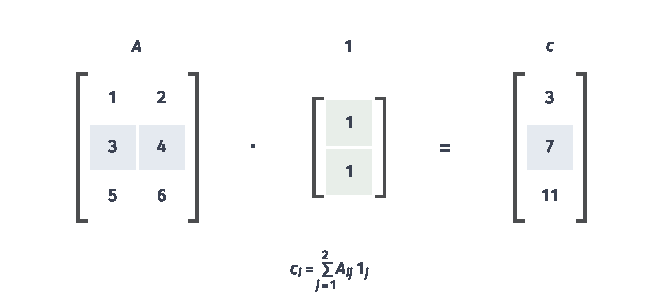
\includegraphics[width=112mm]{figures/00-shared/mathematical-preliminaries-upper/02-linear-spaces/matplotlib/ls-tensor-contraction/ls-tensor-contraction.pdf}
  \caption{张量缩约沿选中的一对轴求和、保留其余轴。左：二阶张量按行和列着色；选中列轴（虚线箭头）沿列求和，输出对每行汇总为一个值。右：缩约后得到$3$个输出，分别对应原矩阵三行的行和，颜色由红（小）经黄到蓝（大）。张量与数值均为解析教学例。}
  \label{fig:ls-tensor-contraction}
\end{figure}

图中对每行求和，也可以看成与全$1$向量沿列轴缩约。前两节的几种运算都是缩约：
\begin{itemize}
 \item 内积$\sum_jx_jy_j$缩约两个向量唯一的一对轴，输出标量；
 \item 矩阵乘法$\sum_\ell a_{i,\ell}b_{\ell,j}$只消去左因子的列轴与右因子的行轴这一对；
 \item 迹$\sum_iA_{i,i}$让同一个矩阵的行轴与列轴共用一个索引，再求和；
 \item Frobenius内积$\sum_{i,j}a_{i,j}b_{i,j}$同时缩约两对轴。
\end{itemize}

\subsubsection{缩约的性质}

缩约只由有限次乘法与求和组成，因此满足以下规则。

\paragraph{线性}
固定参与配对的另一个数组，缩约对被作用的数组是线性的。以示例~\ref{ex:ls-contraction-shapes}（2）中与$\bm W$的缩约为例，把$\bm X$换成$a\bm X+b\bm X'$，
\[
 \sum_{k=1}^d\bigl(a\,x_{i,j,k}+b\,x'_{i,j,k}\bigr)w_{k,t}
 =a\sum_{k=1}^d x_{i,j,k}w_{k,t}+b\sum_{k=1}^d x'_{i,j,k}w_{k,t},
\]
输出变为两个输出的$a$倍与$b$倍之和。一般情形同理：每个输出元素都是被作用数组元素以固定系数作的加权和。

\paragraph{求和次序可交换}
多对轴的缩约是有限和，结果与先消去哪一对轴无关。例如示例~\ref{ex:ls-contraction-shapes}中的$c_{i,j}$，可以先对$s$求和得到中间数组，再对$k$求和，也可以反过来：
\[
 c_{i,j}=\sum_{k=1}^d\Bigl(\sum_{s=1}^r a_{i,k,s}b_{k,j,s}\Bigr)
 =\sum_{s=1}^r\Bigl(\sum_{k=1}^d a_{i,k,s}b_{k,j,s}\Bigr).
\]

\paragraph{简单张量系数可分离}
设一次计算同时依赖三组向量$\bm x\in\mathbb R^m$、$\bm y\in\mathbb R^n$、$\bm z\in\mathbb R^p$。若系数数组是简单张量$\bm a\otimes\bm b\otimes\bm c$，则
\begin{equation}
 \left\langle\bm a\otimes\bm b\otimes\bm c,
 \bm x\otimes\bm y\otimes\bm z\right\rangle_{\mathrm F}
 =(\bm a^\top\bm x)(\bm b^\top\bm y)(\bm c^\top\bm z).
 \label{eq:linear-algebra-rank-one-contraction}
\end{equation}
这是因为$\sum_{i,j,k}a_ib_jc_kx_iy_jz_k=(\sum_ia_ix_i)(\sum_jb_jy_j)(\sum_kc_kz_k)$：三重求和分离成三个内积的乘积，计算量从$mnp$项降到$m+n+p$项。下面用一组小数值核对。
\begin{example}[简单张量系数的分离计算]
\label{ex:ls-rank-one-contraction-check}
取$m=n=p=2$，系数向量为$\bm a=(1,2)^\top$、$\bm b=(3,-1)^\top$、$\bm c=(2,1)^\top$，输入为$\bm x=(2,1)^\top$、$\bm y=(1,1)^\top$、$\bm z=(1,-1)^\top$。按式~\eqref{eq:linear-algebra-rank-one-contraction}右端，只需三个内积：
\[
 \begin{gathered}
 \bm a^\top\bm x=1\cdot2+2\cdot1=4,\qquad
 \bm b^\top\bm y=3\cdot1+(-1)\cdot1=2,\\
 \bm c^\top\bm z=2\cdot1+1\cdot(-1)=1.
 \end{gathered}
\]
三个内积相乘得$4\cdot2\cdot1=8$。若直接展开三重求和，要累加$2^3=8$项、每项是六个数的乘积，结果同样是$8$。分离计算只需对$m+n+p=6$个坐标各做一次乘法，维数增大时，它比逐项展开省下的计算迅速增多。
\end{example}

\paragraph{非线性操作不是缩约}
由上面的线性，固定配对数组的缩约$\mathcal C$满足$\mathcal C(2\bm X)=2\,\mathcal C(\bm X)$。逐元素平方这样的逐元素非线性操作不满足这一点：只要$x_{i,j}\neq0$，
\[
 (2x_{i,j})^2=4x_{i,j}^2\neq2x_{i,j}^2,
\]
所以它不是缩约；$\operatorname{softmax}$等操作同样不是缩约。一个模型若由缩约与这些操作交替组成，那么即使固定了系数、每一步缩约都是线性的，也不能由此推出整个模型是线性的。

\section{本章小结}
\label{sec:ls-operations-summary}

本章按定位一个数所需的索引个数，依次讨论了向量、矩阵与张量的运算。对每种运算，我们都交代了输入条件、输出形状和可用的规则。

向量的加法与数乘逐坐标进行，组合起来就是线性组合。欧氏内积把两个同维向量配成一个数，长度和$p$范数用一个非负数衡量向量的大小。$p$范数非负、正定、齐次，并满足三角不等式，后者由Hölder不等式与Minkowski不等式证明。范数与内积的一般理论分别在第~\ref{chap:normed-spaces}章与第~\ref{chap:inner-product-spaces}章建立。

矩阵乘法来自两次加权求和的复合。它满足结合律与分配律，但不满足交换律与消去律。初等行变换都可以撤销，每一种都等于左乘一个可逆的初等矩阵。

逆矩阵撤销一次乘法：对角矩阵与二阶方阵有直接的求逆公式，一般方阵的求逆归结为解$n$个系数矩阵相同的方程，具体算法留到第~\ref{sec:ls-gaussian-elimination}节。矩阵的幂记录同一矩阵的反复作用。

行列式、迹和Frobenius内积把矩阵变成一个数。行列式是方阵对有向体积的缩放倍数，它非零恰好对应方阵可逆；由古典伴随还可以证明，方阵只要有一侧的逆，这个单侧逆就是逆矩阵。迹只累加对角元素，满足循环性。Frobenius内积配对两个同形矩阵的全部元素，由它得到Frobenius范数。

张量把索引推广到任意多个。重排只改变元素的位置，张量积与Kronecker积保留各因子的全部轴，缩约沿指定的轴求和；内积、矩阵乘法与迹都是缩约的特例。

本章出现了好几种“乘积”，它们的区别在于对索引做什么：有的配对后求和，有的在同一位置相乘而不求和，有的把两组索引全部保留。表~\ref{tab:linear-algebra-products-and-shapes}按这一区别汇总它们的形状条件与输出。遇到一个乘积记号时，先看它消去哪些索引、保留哪些索引，再判断输出的形状与含义。

\begin{table*}[htbp]
 \centering\small
 \begin{tabularx}{\linewidth}{@{}lXX@{}}
  \toprule
  运算 & 形状条件与输出 & 索引作用\\
  \midrule
  $\langle\bm x,\bm y\rangle$ & 两个$n$维向量，输出标量 & 配对后汇总\\
  $\bm A\bm B$ & $(m\times n)(n\times p)\to m\times p$ & 汇总共同索引\\
  $\bm A\odot\bm B$ & 同为$m\times n$，输出仍为$m\times n$ & 同位置相乘，不求和\\
  $\bm x\otimes\bm y$ & $m$维与$n$维向量$\to m\times n$ & 保留两条轴，不求和\\
  $\bm A\otimes\bm B$ & $(m\times n)$与$(p\times q)\to(mp)\times(nq)$ & 保留两组成对索引\\
  缩约 & 被缩约的各对轴长度相同 & 消去指定轴，保留其余轴\\
  \bottomrule
 \end{tabularx}
 \caption{本章各种乘积的形状。同一类乘积记号可能对应不同操作：先看消去哪些索引，再判断输出的形状和含义。}
 \label{tab:linear-algebra-products-and-shapes}
\end{table*}

本章只把这些数组当作具体的数表。第~\ref{chap:linear-representation}章讨论它们记录的是什么：同一个对象换一组方向后坐标怎样改变，矩阵怎样记录线性映射。一般空间中的大小在第~\ref{chap:normed-spaces}章讨论，夹角与正交在第~\ref{chap:inner-product-spaces}章讨论。矩阵乘法的结合律、逆矩阵和幂在后文反复出现：矩阵反复作用的长期行为在第~\ref{chap:linear-recurrence-stability}章讨论，误差经过一次矩阵作用被放大多少在第~\ref{chap:condition-and-spectral-perturbation}章讨论，方程的解与求解方法从第~\ref{chap:linear-solution-selection}章开始讨论。

